\chapter{Experiments}
\label{ChapterExp}

The purpose of the current chapter is, in the first place, to describe in detail the specific tasks and datasets used for the experiments and, in the second place, to show and comment the obtained results.   

\section{Tasks and dataset}
\label{tasks-dataset}

In order to test the model depicted in Section \ref{arch-and-feat}, we considered the following task of the type described in Section \ref{classification}: learning to classify digits from 0 to 9, knowing the sum of $\mathit{n}$ tuples (having cardinality $\mathit{m}$) of them. With reference to the nomenclature used in Section \ref{classification}, let $\mathit{f} = sum(\mathit{c}_1,...,\mathit{c}_m)$ be the function that takes in input $\mathit{m}$ digits from 0 to 9 and compute their sums. Note that such function is not injective (e.g., if $m = 2: 0+3=3$ as well as $2+1=3$) and the order of the elements in the tuple is relevant in the interests of the classification task (e.g., if $m =2: (0,2) \neq (0,2)$ even if $\mathit{f}(0,2) = \mathit{f}(2,0) = 2$).

The starting dataset to perform this task is MNIST, that includes handwritten digits and it is commonly used for training and testing in the filed of machine learning. It contains 60'000 training images and 10'000 testing images; each image has 784 pixels ($28 \times 28$). For the purpose of the experiments, the training set has been split as follows: 54'000 examples for the training set and 6'000 for the validation set. Besides, we removed pixels with very low variance (in particular, where the pixel's variance is smaller than 0.001 times the average variance); the resulting images have 629 pixels. 

\begin{figure}[H]
\caption{Sample images from MNIST dataset.}
\label{fig:mnist}
\centering
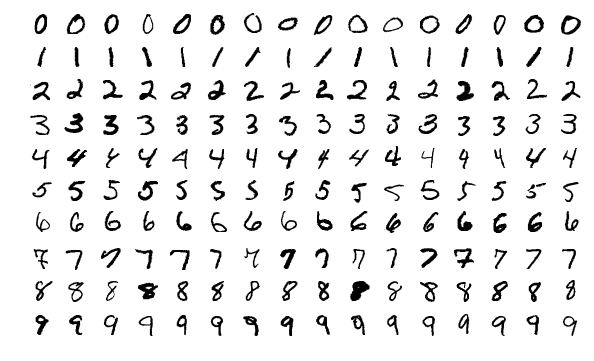
\includegraphics[scale=0.6]{Figures/mnist.png}
\end{figure}
Starting from the dataset just described, we applied the function $\mathit{f}$ to the labels $\mathit{c}_i \in \mathit{C}$ corresponding to observations $\mathbf{x}_i \in \mathit{X}$ in order to modify the dataset in the form $\{((\mathbf{x}_1,...,\mathbf{x}_m),\mathit{f}_1),...,((\mathbf{x}_{n-m+1},...,\mathbf{x}_n),\mathit{f}_{\frac{n}{m}})\}$. In particular, we considered 3 values of $\mathit{m}$ (i.e., number of addends in the sum): 2, 3 and 4. Increasing such a value makes the task harder for two reasons:

\begin{itemize}
  \item the number of possible abductions increases, with equal sum. For example: if $sum(\mathit{c}_1,\mathit{c}_2) = 2$, then $\mathit{A}$ = \{(0,2), (1,1), (2,0)\} and $|\mathit{A}| = 3$; if $sum(\mathit{c}_1,\mathit{c}_2,\mathit{c}_3) = 2$, then $\mathit{A}$ = \{(0,0,2), (0,2,0), (2,0,0), (1,1,0), (1,0,1), (0,1,1)\} and $|\mathit{A}| = 6$;
  \item the number of observed cases in the modified dataset in which there is only one possible abduction decreases. In order to explain this observation, let us first consider the case of $m = 2$. The cases in which we have just one possible abduction are when the sum is 0 or 18; in fact, in such cases, we know that the possible addends are respectively only (0,0) and (9,9). Considering $m = 3$, we can make the same argument for sums 0 and 27. The difference lies in the way in which the modified dataset is computed: since we apply the function $\mathit{f} = sum(\mathit{c}_1,...,\mathit{c}_m)$ to the labels $\mathit{c}_i \in \mathit{C}$, the cases in which we have $m = 3$ zero (or equivalently nine) in succession decreases. Similarly, this number goes on to decrease when we consider $m = 4$.
\end{itemize}
Basically, we want to evaluate the model making the task more and more difficult, that is decreasing the number of observed certainties (i.e., cases in which there is only one possible abduction) and increasing the number of possible abductions. 
 
These considerations are highlighted in Table \ref{tab:info-tasks}, which shows the number of examples and the corresponding number of possible abductions by varying the value of $m$. We can observe that the certainties decrease from 1048 when $m = 2$ to 102 when $m = 3$ to only 12 when $m = 4$. Besides, we underline the significative increse of possible abductions for examples.

\begin{table}[H]
  \centering
  \caption{Number of examples and corresponding number of possible abductions respectively for $m = 2$, $m = 3$ and $m = 4$ for dataset MNIST. Rows in bold highlight the certainties for each task.}
  \label{tab:info-tasks}
  \scriptsize
  \begin{tabular}[t]{ll}
    \toprule
    \#(ex)	& \#(abd)\\
    \midrule
    \textbf{1048}	& \textbf{1}\\
    2480			& 2\\
	3228			& 3\\
	4580			& 4\\
	5278			& 5\\
	6398			& 6\\
	7332			& 7\\
	8640			& 8\\
	9744			& 9\\
	5272			& 10\\
    \bottomrule
  \end{tabular}
  \qquad
  \scriptsize
  \begin{tabular}[t]{ll}
    \toprule
    \#(ex)	& \#(abd)\\
    \midrule
    \textbf{102}	& \textbf{1}\\
    459				& 3\\
	684				& 6\\
	1305			& 10\\
	1788			& 15\\
	2625			& 21\\
	2961			& 28\\
	3927			& 36\\
	4803			& 45\\
	5952			& 55\\
	6585			& 63\\
	7269			& 69\\
	7707			& 73\\
	7833			& 75\\
    \bottomrule
  \end{tabular}
    \qquad
  \scriptsize
  \begin{tabular}[t]{ll}
    \toprule
    \#(ex)	& \#(abd)\\
    \midrule
    \textbf{12}		& \textbf{1}\\
    40				& 4\\
	164				& 10\\
	296				& 20\\
	412				& 35\\
	708				& 56\\
	1104			& 84\\
	1468			& 120\\
	1836			& 165\\
	2452			& 220\\
	3164			& 282\\
	3776			& 348\\
	4556			& 415\\
	5288			& 480\\
	5824			& 540\\
	6484			& 592\\
	6336			& 633\\
	6636			& 660\\
	3444			& 670\\
    \bottomrule
  \end{tabular}
\end{table}

\section{Results}
\label{results}
In the following, we show and analyse the experiments results on the tree tasks described in Section \ref{tasks-dataset}. According to the specific task and related difficulties, we performed a grid search by varying the model hyper-parameters, which are in summary:

\begin{itemize}
	\item split-depth, number of input distributions, number of root nodes, number of sum nodes per inner regions, dropout at input, dropout at sums (from RAT-SPN, see Section \ref{rat-spn});
	\item abductions threshold and pre-training (see Sections \ref{abd-threshold} and \ref{clustering}).
\end{itemize}
On the contrary, we fixed the batch size and the number of epochs to $100$ and the use of \textit{adam} (adaptive moment estimation) \cite{kingma2017adam} as optimization algorithm for RAT-SPN.

\subsection{Sum of pairs}
\label{results-pairs}
Table \ref{tab:results-pairs} shows the esperiments results in the case of $m=2$ (i.e., sum of pairs). Because of the training computational cost of RAT-SPNs with split depth striclty greater than 1, we tested only the configurations with split depth equal to 1, exploring almost all the ones proposed by Peharz et al. \cite{DBLP:journals/corr/abs-1806-01910} in the original experiments on mnist dataset (only configurations with dropout equal to 0.25 have been discarded, given th reduced dimension of the considered SPNs). As regards the introduced hyper-parameters (i.e., abduction threshold and pre-training), since the task under consideration presents a sufficiently high number of "certainties" (i.e., observations with just one possible abduction) and a not so significant number of possible abductions (see Table \ref{tab:info-tasks}), we decided not to exploit these additional implemented features in this case (i.e., threshold = 0 and pre-training = false).

\begin{table}[H]
  \centering
  \caption{Performance for $\mathit{f} = sum(\mathit{c}_1,\mathit{c}_2)$. Batch size = $100$, number of epochs = $100$, optimization algorithm: \textit{adam}, abductions threshold = 0, pre-training = false. All accuracy values are in percentage and approximated to the second digit after the decimal place. The best configuration is highlighted in bold.}
  \label{tab:results-pairs}
  \tiny
  \begin{tabular}{ccccccrr}
    \toprule
    depth		& distributions 	& splits 		& sums 				& dropout input 		& dropout sums 			& valid acc 			& test acc\\
    \midrule
    1      		& 10     			& 9      		& 10     			& 1      				& 1      				& 94.87    				& 94.74\\ 
    1      		& 10     			& 9      		& 10     			& 1      				& 0.75    				& 94.77    				& 94.8\\ 
    1      		& 10     			& 9      		& 10     			& 1      				& 0.50    				& 95.27    				& 94.84\\	
	1      		& 10     			& 9      		& 10     			& 0.75    				& 1      				& 96.07    				& 95.77\\
	1      		& 10     			& 9      		& 10     			& 0.75    				& 0.75    			    & 96.18    				& 95.76\\         
    1      		& 10     			& 9      		& 10     			& 0.75    				& 0.50    				& 96.53    				& 95.91\\ 
    1      		& 10     			& 9      		& 10     			& 0.50    				& 1      				& 96.17				    & 95.89\\
	1      		& 10     			& 9      		& 10     			& 0.50    				& 0.75    				& 96.38    				& 95.90\\   
    1      		& 10				& 9			    & 10				& 0.50					& 0.50					& 96.07    				& 95.82\\
 
	1      		& 15     			& 14     		& 10     			& 1      				& 1      				& 94.90				    & 95.43\\ 
	1      		& 15     			& 14     		& 10     			& 1      				& 0.75    				& 95.57    				& 95.57\\
	1      		& 15     			& 14     		& 10     			& 1      				& 0.50    				& 95.12    				& 95.30\\ 
	1      		& 15     			& 14     		& 10     			& 0.75    				& 1      				& 96.57				    & 96.23\\  
	1      		& 15     			& 14     		& 10     			& 0.75    				& 0.75    				& 96.48    				& 96.36\\
	1      		& 15     			& 14     		& 10     			& 0.75   	 			& 0.50    				& 96.72    				& 96.27\\ 
	1      		& 15     			& 14     		& 10     			& 0.50    				& 1      			    & 96.53    				& 96.08\\
	1      		& 15     			& 14     		& 10     			& 0.50    				& 0.75    				& 96.63    				& 96.17\\  
	1      		& 15     			& 14     		& 10     			& 0.50    				& 0.50    				& 96.33    				& 95.99\\ 

	1      		& 20     			& 19     		& 10     			& 1      				& 1      				& 95.60    				& 95.59\\ 
	1      		& 20     			& 19     		& 10     			& 1      				& 0.75					& 95.37				    & 95.45\\ 
	1      		& 20     			& 19     		& 10     			& 1      				& 0.50					& 95.63    				& 95.22\\
	1      		& 20     			& 19     		& 10     			& 0.75    				& 1     				& 96.88    				& 96.58\\  
	1		    & 20     			& 19     		& 10     			& 0.75    				& 0.75				    & 96.60    				& 96.47\\ 
	1      		& 20     			& 19     		& 10     			& 0.75    				& 0.50    				& 96.57					& 96.67\\
	1      		& 20     			& 19     		& 10     			& 0.50    				& 1						& 96.95   				& 96.48\\ 
	1      		& 20     			& 19     		& 10     			& 0.50    				& 0.75    				& 96.52    				& 96.28\\ 
	1      		& 20     			& 19     		& 10     			& 0.50    				& 0.50    				& 96.75    				& 96.19\\ 

	1      		& 25     			& 29     		& 10     			& 1      				& 1      				& 95.90    				& 95.80\\
	1	      	& 25     			& 29     		& 10     			& 1      				& 0.75    				& 95.83    				& 95.73\\
	1      		& 25     			& 29     		& 10     			& 1      				& 0.50    				& 95.62					& 95.90\\
	1      		& 25     			& 29     		& 10     			& 0.75    				& 1      				& 96.93    				& 96.51\\
 	1      		& 25     			& 29     		& 10     			& 0.75    				& 0.75    				& 96.72    				& 96.63\\ 
	1      		& 25     			& 29     		& 10     			& 0.75    				& 0.50    				& 96.87					& 96.76\\
	1      		& 25     			& 29     		& 10     			& 0.50    				& 1      				& 96.82    				& 96.73\\ 
	1      		& 25     			& 29     		& 10     			& 0.50    				& 0.75    				& 96.95				    & 96.60\\
	1      		& 25     			& 29     		& 10     			& 0.50   				& 0.50    				& 96.67				    & 96.50\\

	1      		& 33     			& 40     		& 10     			& 1      				& 1      				& 95.97    				& 95.67\\
	1      		& 33     			& 40     		& 10     			& 1      				& 0.75    				& 95.78    				& 95.93\\
	1      		& 33     			& 40     		& 10     			& 1      				& 0.50    				& 95.77    				& 95.71\\
	1      		& 33    			& 40     		& 10     			& 0.75    				& 1      				& 96.77    				& 96.51\\
	1      		& 33     			& 40    		& 10     			& 0.75    				& 0.75    				& 96.77    				& 96.66\\ 	
	1      		& 33     			& 40     		& 10     			& 0.75				    & 0.50				    & 96.90				    & 96.48\\ 
	1      		& 33     			& 40     		& 10     			& 0.50    				& 1      				& 97.03    				& 96.89\\ 
	1      		& 33     			& 40     		& 10     			& 0.50    				& 0.75					& 96.95					& 96.87\\ 			
	\textbf{1} 	& \textbf{33}     	& \textbf{40}   & \textbf{10}		& \textbf{0.50}    		& \textbf{0.50}    		& \textbf{97.10}    	& \textbf{96.88}\\
    \bottomrule
  \end{tabular}
\end{table}

\newpage
First of all, we observe that accuracy values are very similar among all the considered configurations, in contrast with the model showed in Section \ref{challenge}. This means that the labeling accuracy (hence the training success) does not depend on the chance, but on a deterministic learning, that always carries out the model to understand (more or less according to the specific configuration and only in a very small part to the chance) the proper "direction" to take. In conclusion, we can infer that, for this specific task, the only observations sorting mechanism (described in Section \ref{sorting}) turns out to be sufficient in order to achieve great performance.

\subsection{Sum of triples}
Table \ref{tab:results-triples-clno} and \ref{tab:results-triples-clyes} show the esperiments results in the case of $m=3$ (i.e., sum of triples). Since in the previous experiment (Section \ref{results-pairs}) no significant difference was observed increasing the number of input distributions and since we are more interested in understanding the model behaviour than the real performance in terms of accuracy, we explored the ones having less computational cost. In this case, however, given the increased difficulty (see Table \ref{tab:info-tasks}) we introduced both the abduction threshold and the pre-training. 

\begin{table}[H]
  \centering
  \caption{Performance for $\mathit{f} = sum(\mathit{c}_1,\mathit{c}_2,\mathit{c}_3)$. Batch size = $100$, number of epochs = $100$, optimization algorithm: \textit{adam}, \textbf{pre-training = false}. All accuracy values are in percentage and approximated to the second digit after the decimal place. The best configuration is highlighted in bold.}
  \label{tab:results-triples-clno}
  \scriptsize
  \begin{tabular}{cccccccrr}
    \toprule
    depth		& distributions 	& splits 		& sums 				& dropout input 		& dropout sums 			& threshold				& valid acc 			& test acc\\
    \midrule
	1      		& 10     			& 9      		& 10     			& 1      				& 1      				& 0      				& 94.10    				& 94.19\\ 
	1      		& 10     			& 9				& 10     			& 1      				& 1      				& 0.01    				& 98.05    			    & 94.22\\ 
	1      		& 10     			& 9      		& 10     			& 1      				& 1      				& 0.05    				& 94.47    				& 94.30\\
	1      		& 10     			& 9      		& 10     			& 1      				& 1      				& 0.10    				& 94.35    				& 94.35\\
    1      		& 10     			& 9      		& 10     			& 0.75    				& 0.75    				& 0      				& 96.78    				& 96.46\\
	1      		& 10     			& 9      		& 10     			& 0.75    				& 0.75    				& 0.05    				& 96.27    				& 95.89\\
	1      		& 10     			& 9      		& 10     			& 0.75    				& 0.75    				& 0.01    				& 96.63    				& 96.21\\ 
	1      		& 10     			& 9      		& 10     			& 0.75    				& 0.75    				& 0.10    				& 95.82    				& 95.45\\ 

	1      		& 15     			& 14     		& 10     			& 1      				& 1      				& 0      				& 94.22    				& 94.52\\
	1      		& 15     			& 14     		& 10     			& 1      				& 1      				& 0.01    				& 95.23    				& 94.63\\ 		
	1      		& 15     			& 14     		& 10     			& 1      				& 1      				& 0.05    				& 94.67    				& 94.66\\
	1      		& 15     			& 14     		& 10     			& 1      				& 1      				& 0.10    				& 98.14					& 94.71\\
	1      		& 15     			& 14     		& 10     			& 0.75    				& 0.75    				& 0      				& 96.85					& 96.14\\ 
	1      		& 15     			& 14     		& 10     			& 0.75					& 0.75					& 0.01					& 96.00    				& 95.57\\ 
	1      		& 15     			& 14     		& 10     			& 0.75    				& 0.75    				& 0.05    				& 96.63    				& 96.34\\ 
	1      		& 15     			& 14     		& 10     			& 0.75    				& 0.75    				& 0.10    				& 95.52    				& 95.49\\ 

	\textbf{1}  & \textbf{20}     	& \textbf{19}	& \textbf{10}		& \textbf{1}			& \textbf{1}      		& \textbf{0}      		& \textbf{98.52} 		& \textbf{94.78}\\ 
	1      		& 20     			& 19     		& 10     			& 1      				& 1      				& 0.01    				& 94.73    				& 94.59\\ 
	1      		& 20     			& 19     		& 10     			& 1      				& 1      				& 0.05    				& 94.62    				& 94.68\\
	1      		& 20     			& 19     		& 10     			& 1      				& 1      				& 0.10    				& 95.13    				& 94.66\\
	1      		& 20     			& 19     		& 10     			& 0.75      			& 0.75      			& 0	    				& 96.27    				& 96.10\\
	1      		& 20     			& 19     		& 10     			& 0.75      			& 0.75      			& 0.01    				& 96.87    				& 96.29\\
	1      		& 20     			& 19     		& 10     			& 0.75      			& 0.75      			& 0.05    				& 96.63    				& 96.35\\
	1      		& 20     			& 19     		& 10     			& 0.75      			& 0.75      			& 0.10    				& 96.83    				& 96.58\\
    \bottomrule
  \end{tabular}
\end{table}

\begin{table}[H]
  \centering
  \caption{Performance for $\mathit{f} = sum(\mathit{c}_1,\mathit{c}_2,\mathit{c}_3)$. Batch size = $100$, number of epochs = $100$, optimization algorithm: \textit{adam}, \textbf{pre-training = true}. All accuracy values are in percentage and approximated to the second digit after the decimal place. The best configuration is highlighted in bold.}
  \label{tab:results-triples-clyes}
  \scriptsize
  \begin{tabular}{cccccccrr}
    \toprule
    depth		& distributions 	& splits 		& sums 				& dropout input 		& dropout sums 			& threshold				& valid acc 			& test acc\\
    \midrule
	1      		& 10     			& 9      		& 10     			& 1      				& 1      				& 0      				& 94.05    				& 94.23\\ 
	1      		& 10     			& 9				& 10     			& 1      				& 1      				& 0.01    				& 94.65    			    & 94.24\\ 
	1      		& 10     			& 9      		& 10     			& 1      				& 1      				& 0.05    				& 94.17    				& 94.37\\
	1      		& 10     			& 9      		& 10     			& 1      				& 1      				& 0.10    				& 94.23    				& 94.02\\
    1      		& 10     			& 9      		& 10     			& 0.75    				& 0.75    				& 0      				& 96.50    				& 95.87\\
	1      		& 10     			& 9      		& 10     			& 0.75    				& 0.75    				& 0.05    				& 96.32    				& 95.96\\
	1      		& 10     			& 9      		& 10     			& 0.75    				& 0.75    				& 0.01    				& 96.38    				& 96.08\\ 
	1      		& 10     			& 9      		& 10     			& 0.75    				& 0.75    				& 0.10    				& 96.08    				& 95.86\\ 

	1      		& 15     			& 14     		& 10     			& 1      				& 1      				& 0      				& 94.80   				& 94.79\\
	1      		& 15     			& 14     		& 10     			& 1      				& 1      				& 0.01    				& 95.00    				& 94.96\\ 		
	1      		& 15     			& 14     		& 10     			& 1      				& 1      				& 0.05    				& 95.02    				& 94.92\\
	1      		& 15     			& 14     		& 10     			& 1      				& 1      				& 0.10    				& 94.43					& 94.08\\
	1      		& 15     			& 14     		& 10     			& 0.75    				& 0.75    				& 0      				& 96.80					& 96.25\\ 
	1      		& 15     			& 14     		& 10     			& 0.75					& 0.75					& 0.01					& 96.37    				& 95.41\\ 
	1      		& 15     			& 14     		& 10     			& 0.75    				& 0.75    				& 0.05    				& 96.57    				& 96.13\\ 
	1      		& 15     			& 14     		& 10     			& 0.75    				& 0.75    				& 0.10    				& 96.57    				& 96.40\\ 

	1  			& 20     			& 19			& 10				& 1						& 1      				& 0      				& 95.13 				& 94.59\\ 
	1      		& 20     			& 19     		& 10     			& 1      				& 1      				& 0.01    				& 94.88    				& 95.26\\ 
	1      		& 20     			& 19     		& 10     			& 1      				& 1      				& 0.05    				& 95.02    				& 95.14\\
	1      		& 20     			& 19     		& 10     			& 1      				& 1      				& 0.10    				& 95.13    				& 94.87\\
	\textbf{1}  & \textbf{20}     	& \textbf{19}   & \textbf{10}     	& \textbf{0.75}      	& \textbf{0.75}      	& \textbf{0}	    	& \textbf{96.88}    	& \textbf{96.15}\\
	1      		& 20     			& 19     		& 10     			& 0.75      			& 0.75      			& 0.01    				& 96.82    				& 96.38\\
	1      		& 20     			& 19     		& 10     			& 0.75      			& 0.75      			& 0.05    				& 96.70    				& 96.47\\
	1      		& 20     			& 19     		& 10     			& 0.75      			& 0.75      			& 0.10    				& 96.80    				& 96.45\\
    \bottomrule
  \end{tabular}
\end{table}
As with the case of $m=2$, we can notice the same constant behaviour (in terms of accuracy) among the tested configurations. Such consideration confirms that, also in the case of a task that is more difficult than the previous one, the learning process is deterministic. As regards the abduction threshold, its use doesn't seem to bring advantages to the model, from a purely perfomance point of view; the best observed configurations (highlighted in bold) actually work without threshold (i.e., equal to 0). Analogous observation can be done for the pre-training: even if the best configuration of the pre-trained model performs better on the test set with respect to the best of the not pre-trained one, the comparison between correspondent configurations points out a substancial similarity. Nevertheless, it is interesting to see if some differences come out in the general model behaviour by varying the threshold value and enabling the pre-training. To this end, Figures \ref{fig:thresholds-triples} show \textit{(i)} the number of considered examples, \textit{(ii)} the examples labeling accuracy (to perform the successive training) and \textit{(iii)} the model accuracy on validation set per epoch, by varying the abduction threshold and enabling the pre-training. We can make the following observations:

\begin{itemize}
	\item the greater the threshold, the more the number of considered examples increases slowly; of course, when the threshold is equal to 0, all examples are taken into account from the first epoch to the last one. Besides, when the pre-training is enabled, much more examples are considered from the beginning and the number of considered examples increases faster, since the initialization of the model is no longer randomic;
	\item in the case of threshold uqual to 0.05 and 0.1 without pre-training, the examples labeling accuracy starts from the top value (since it considers all and only the examples with just one possible abduction), but then it drops to very small values, because the low number of considered examples was not sufficient to learn enough. Nevertheless, in both cases, the model is able to improve again its examples labeling accuracy and to easily overcome the model without threshold (i.e., equal to 0) after some epochs. When pre-training is enabled, the model directly starts from low values of labeling accuracy, since it considers more examples from the beginning, and it again learns faster than the model wituout threshold. The motivation behind such improvement definitely lies in the fact the such threshold values allow the model to label (and consequenlty consider) examples with a certain degree of certainty. On the contrary, when the threshold is set to 0.01, no advantage is observed, actually the no threshold model performs better;
	\item the model accuracy behaviour on validation set is very similar to the examples labeling accuracy one (except for the drop in the case of thresholds 0.05 and 0.1 and disabled pre-training). The motivation of such observation lies in the way in which the most probable abduction is selected (see \ref{abd-selection}): since this choice depends on the sub-symbolic model, the more it is learning, the more its accuracy increases both on the validation set and in selecting the abduction for the training examples.
\end{itemize}
In the light of the above considerations, we can conclude that, although all configurations achieve good performance in terms of accuracy, the use both of a sufficiently high threshold and of the pre-training allows the model to converge faster, even if starting from lower accuracy values.

\begin{figure}[H]
\captionsetup{font={small, stretch=1.3}}
\caption{Behaviour comparison between the not pre-trained model and the pre-trained one for $\mathit{f} = sum(\mathit{c}_1,\mathit{c}_2,\mathit{c}_3)$, taking into account: number of considered examples, examples labeling accuracy and model accuracy on validation set per epoch by varying the abduction threshold. The average values have been computed among different configurations but with the same threshold.}
\label{fig:thresholds-triples}
{\setlength{\tabcolsep}{1pt}
\renewcommand*{\arraystretch}{0.6}
\begin{longtable}{cc}
\textbf{Pre-training = false} & \textbf{Pre-training = true} \\
\subfloat{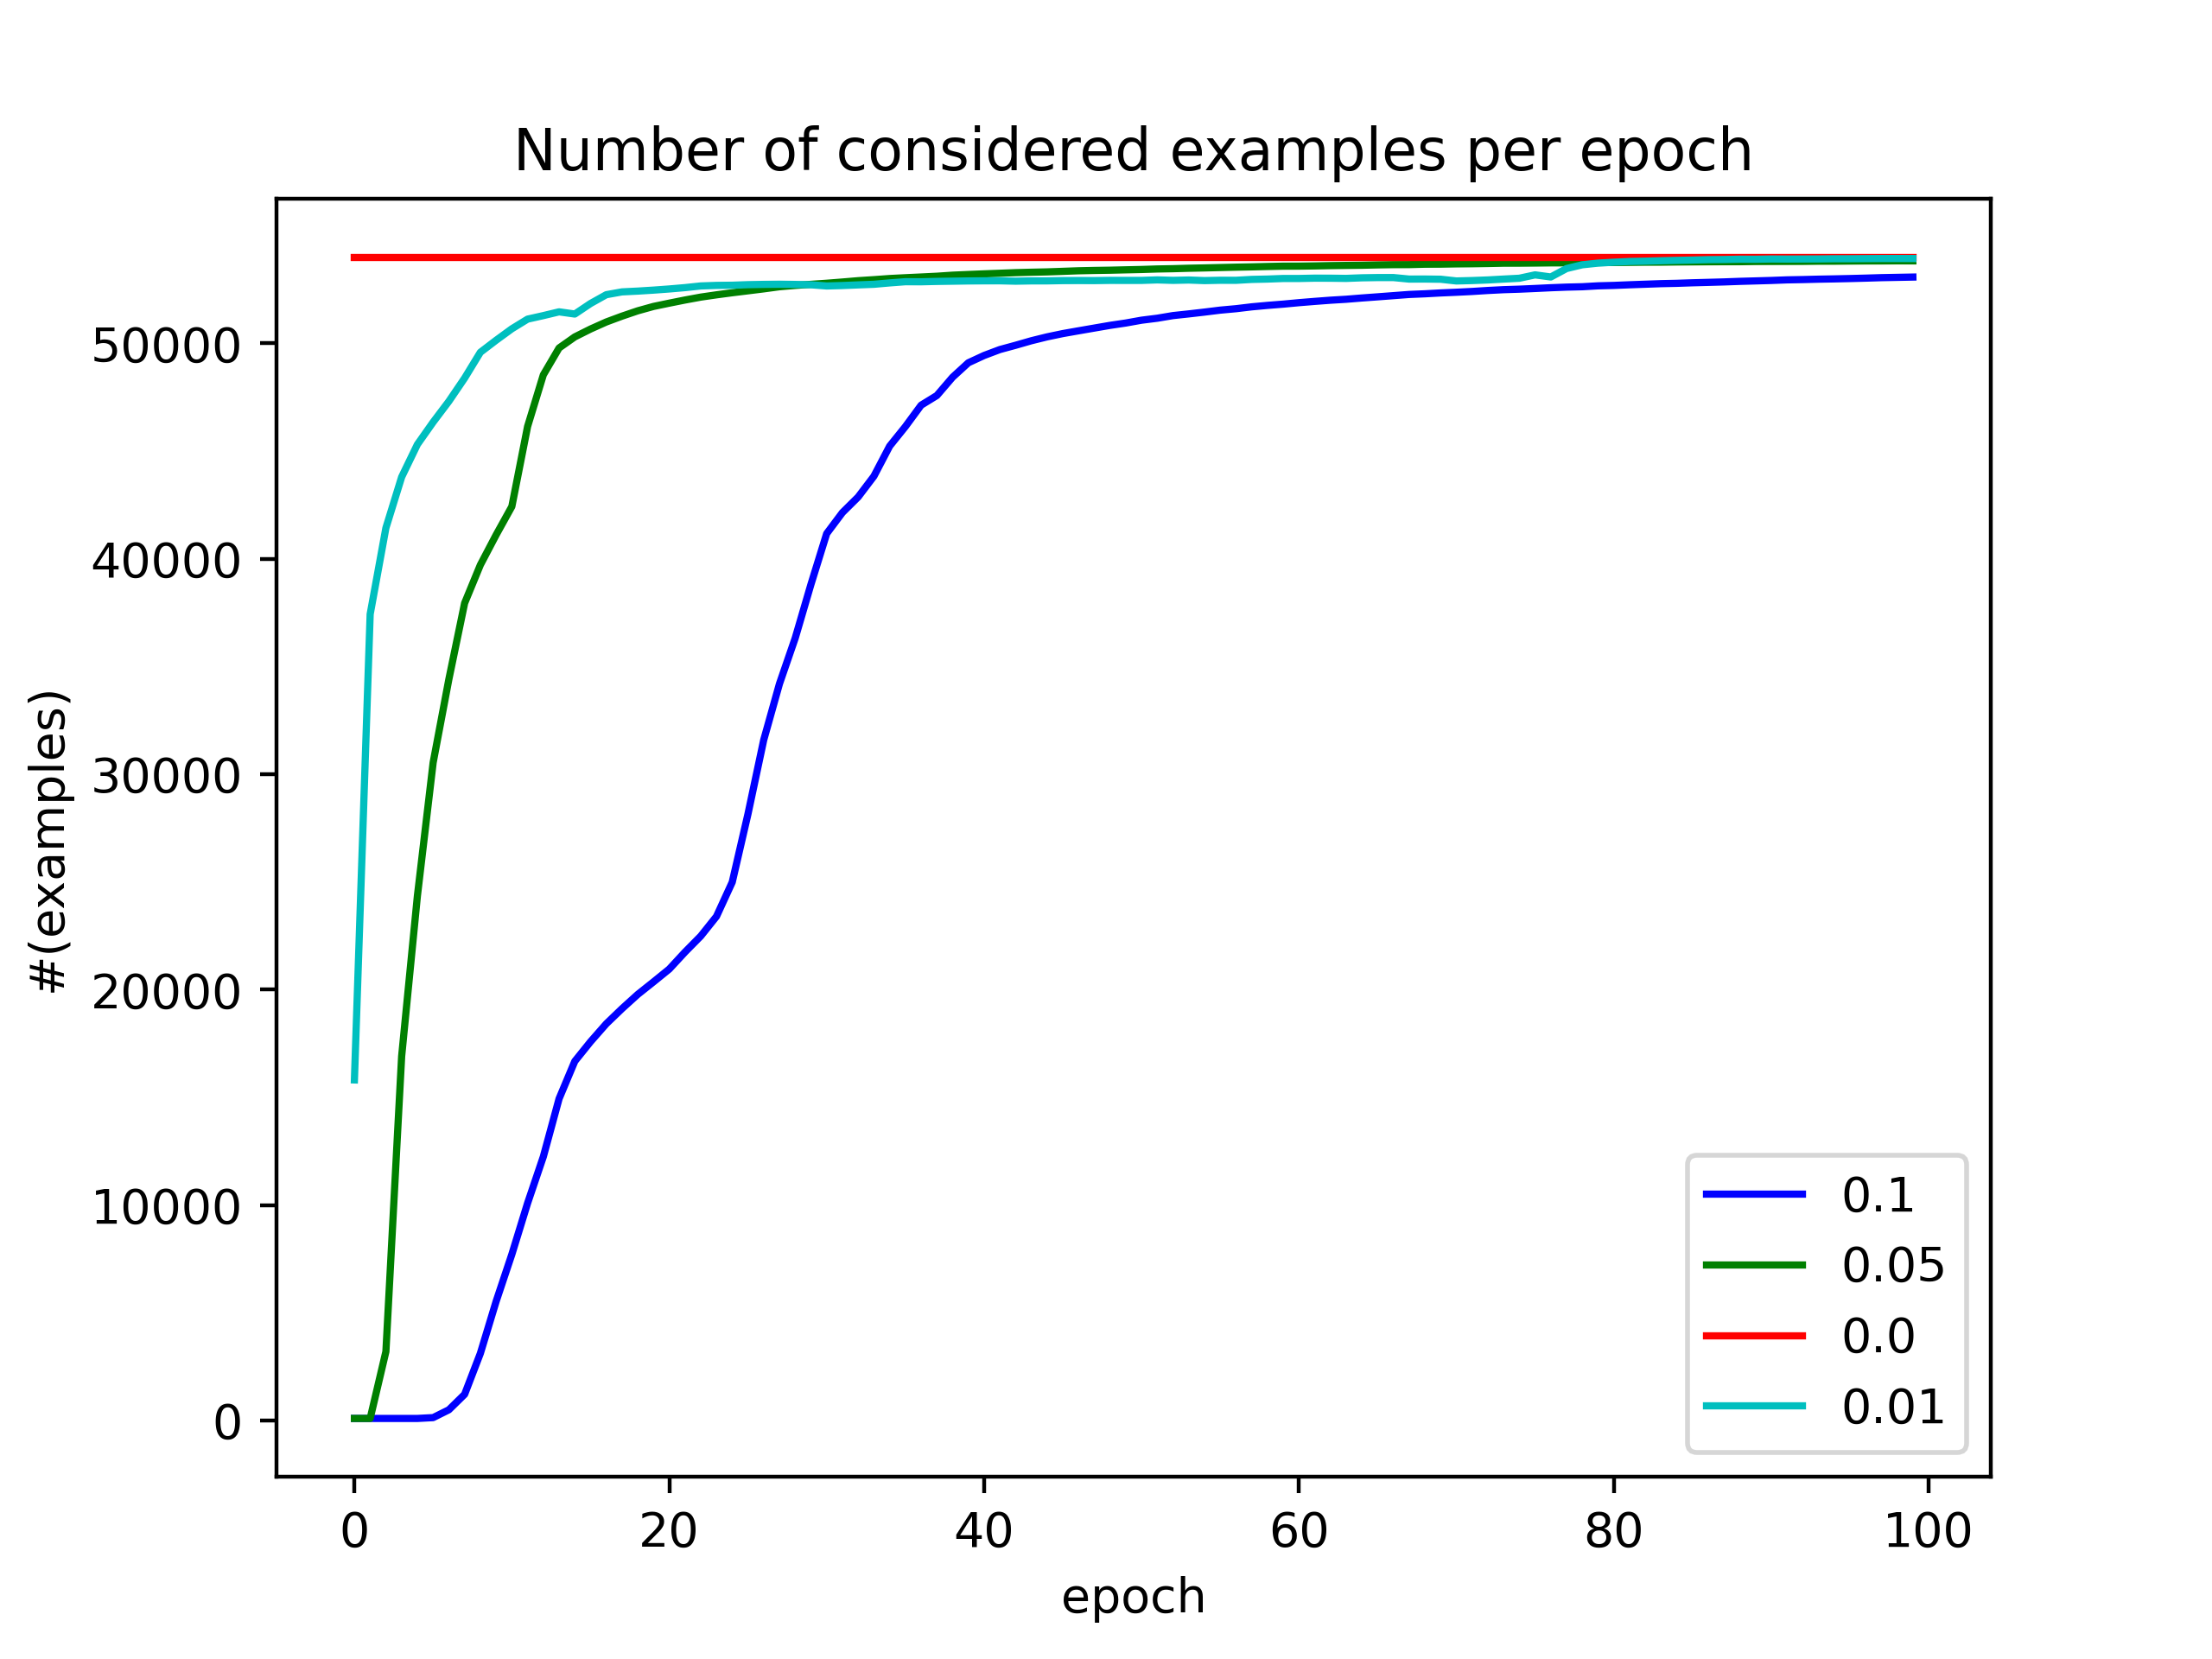
\includegraphics[scale=0.45]{Figures/num_addends_3/examples_clno.png}} & 
\subfloat{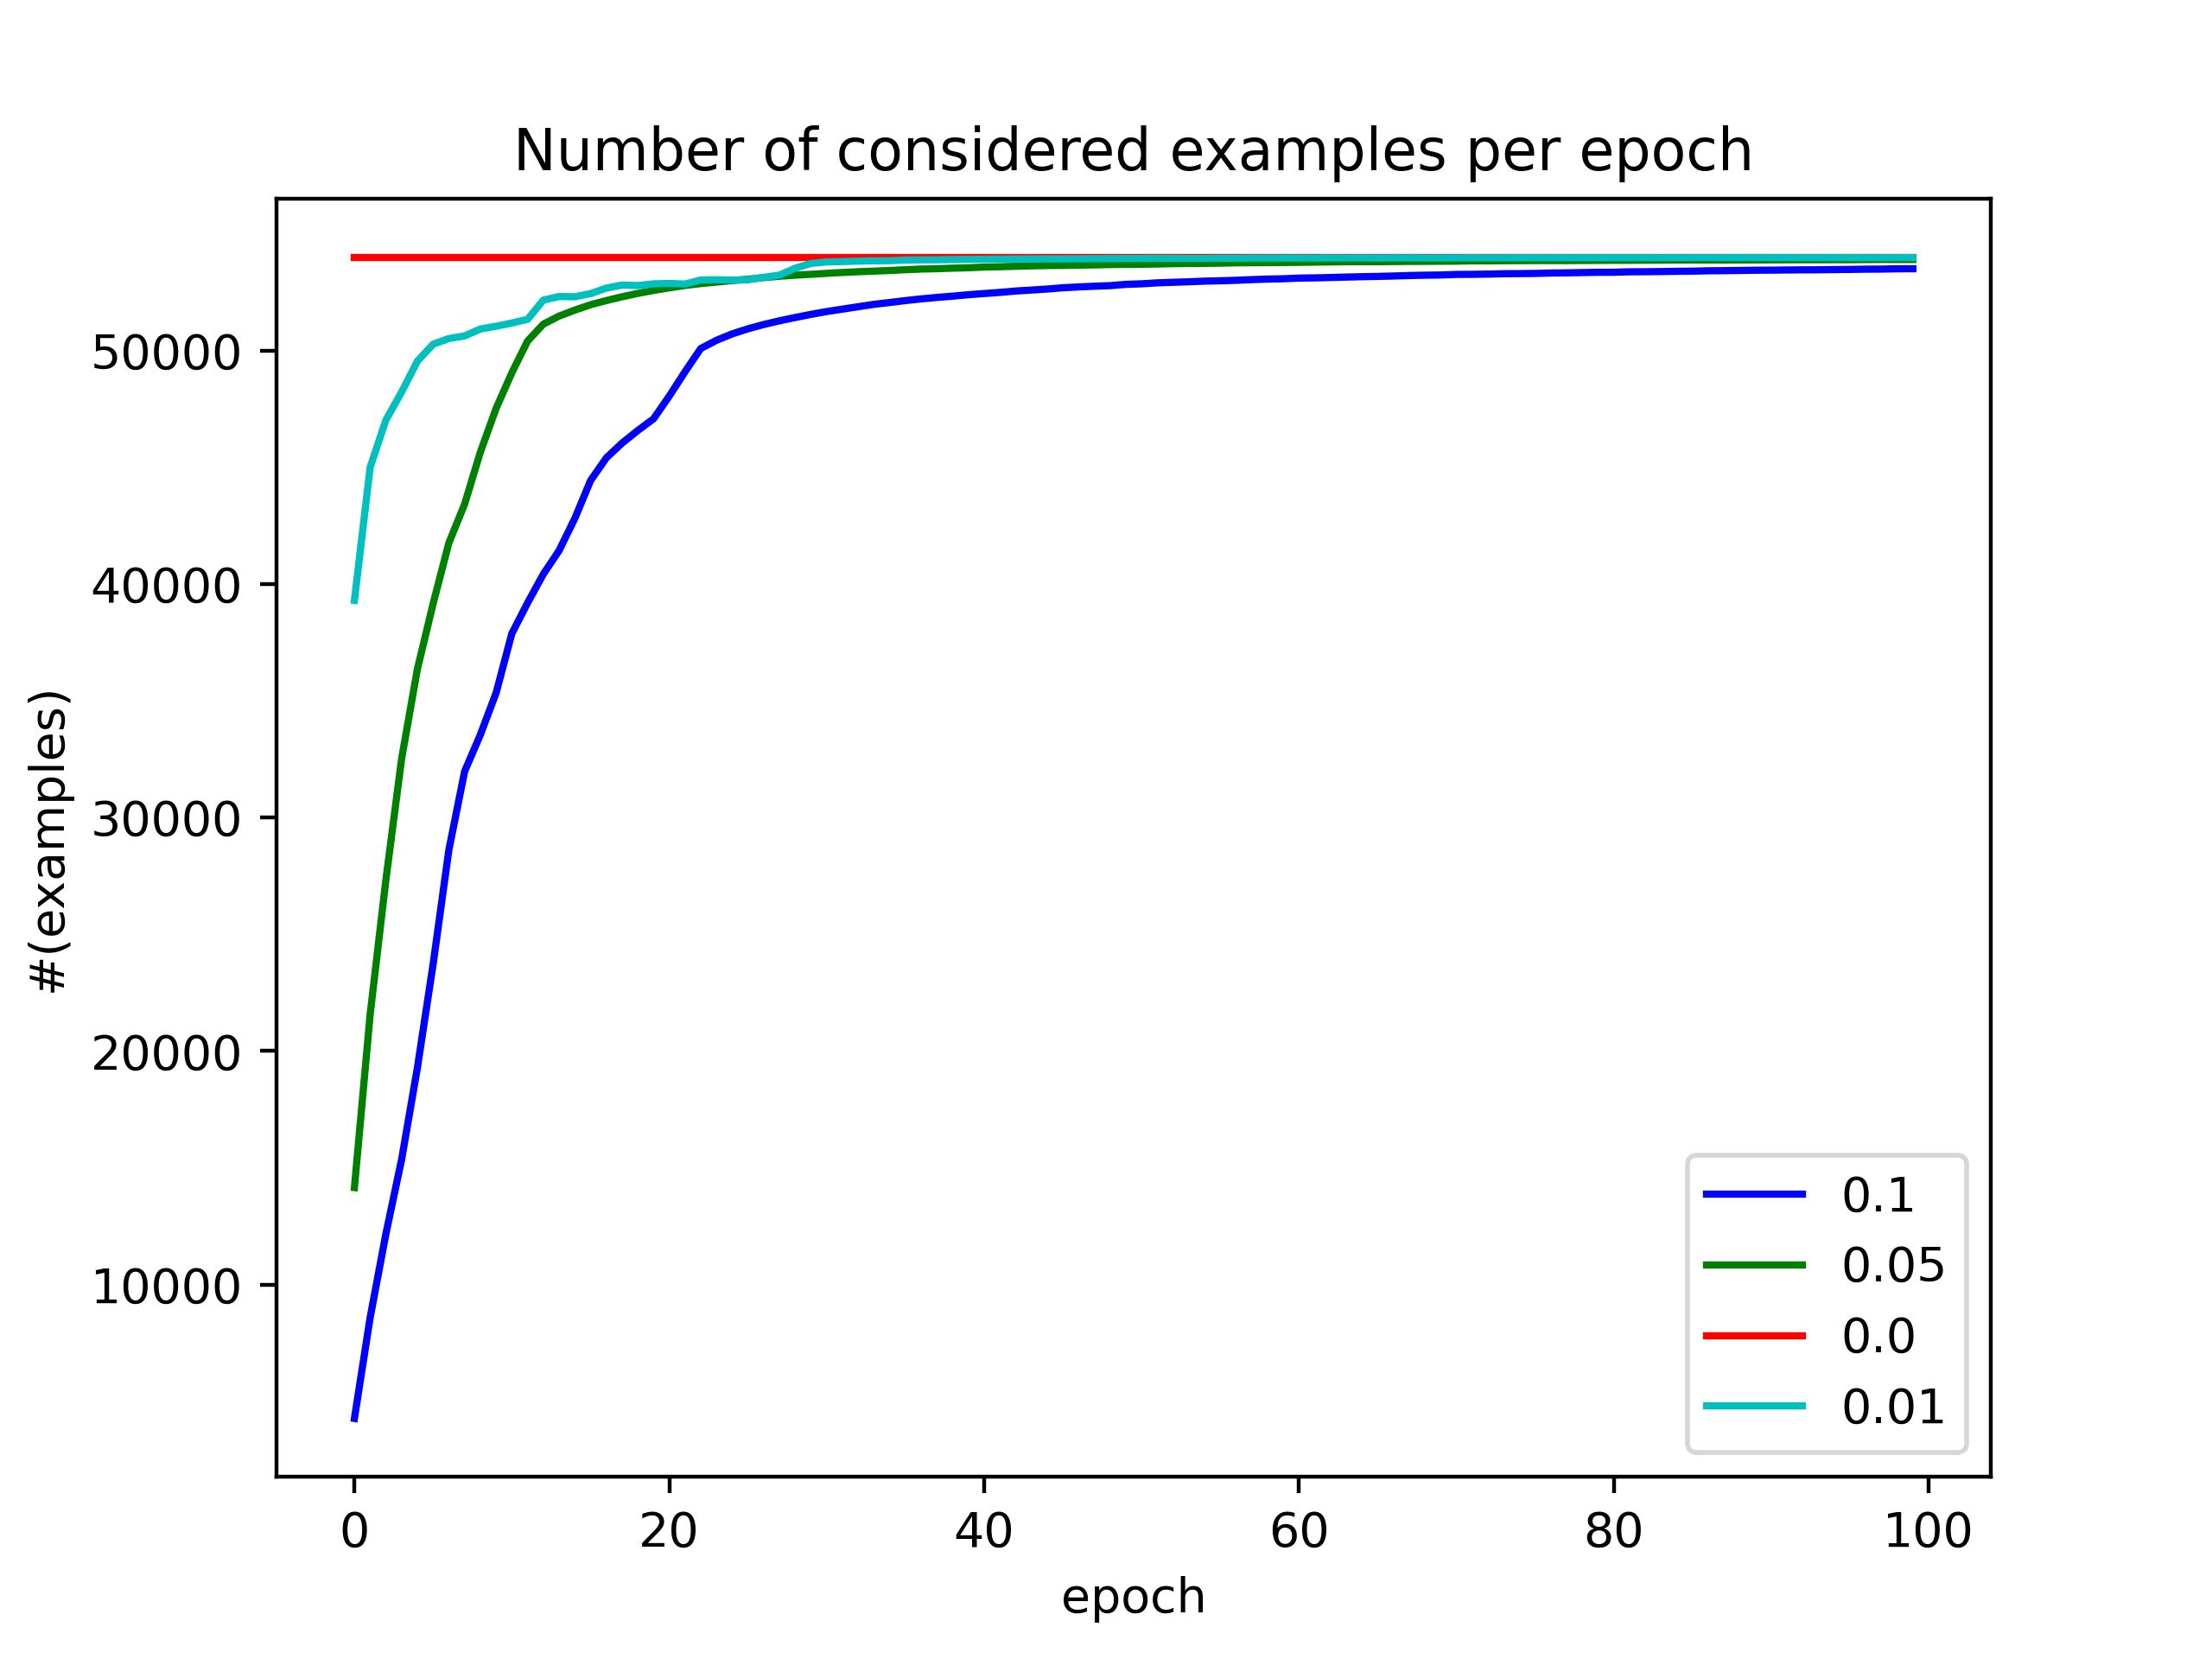
\includegraphics[scale=0.45]{Figures/num_addends_3/examples_clyes.png}} \\

\subfloat{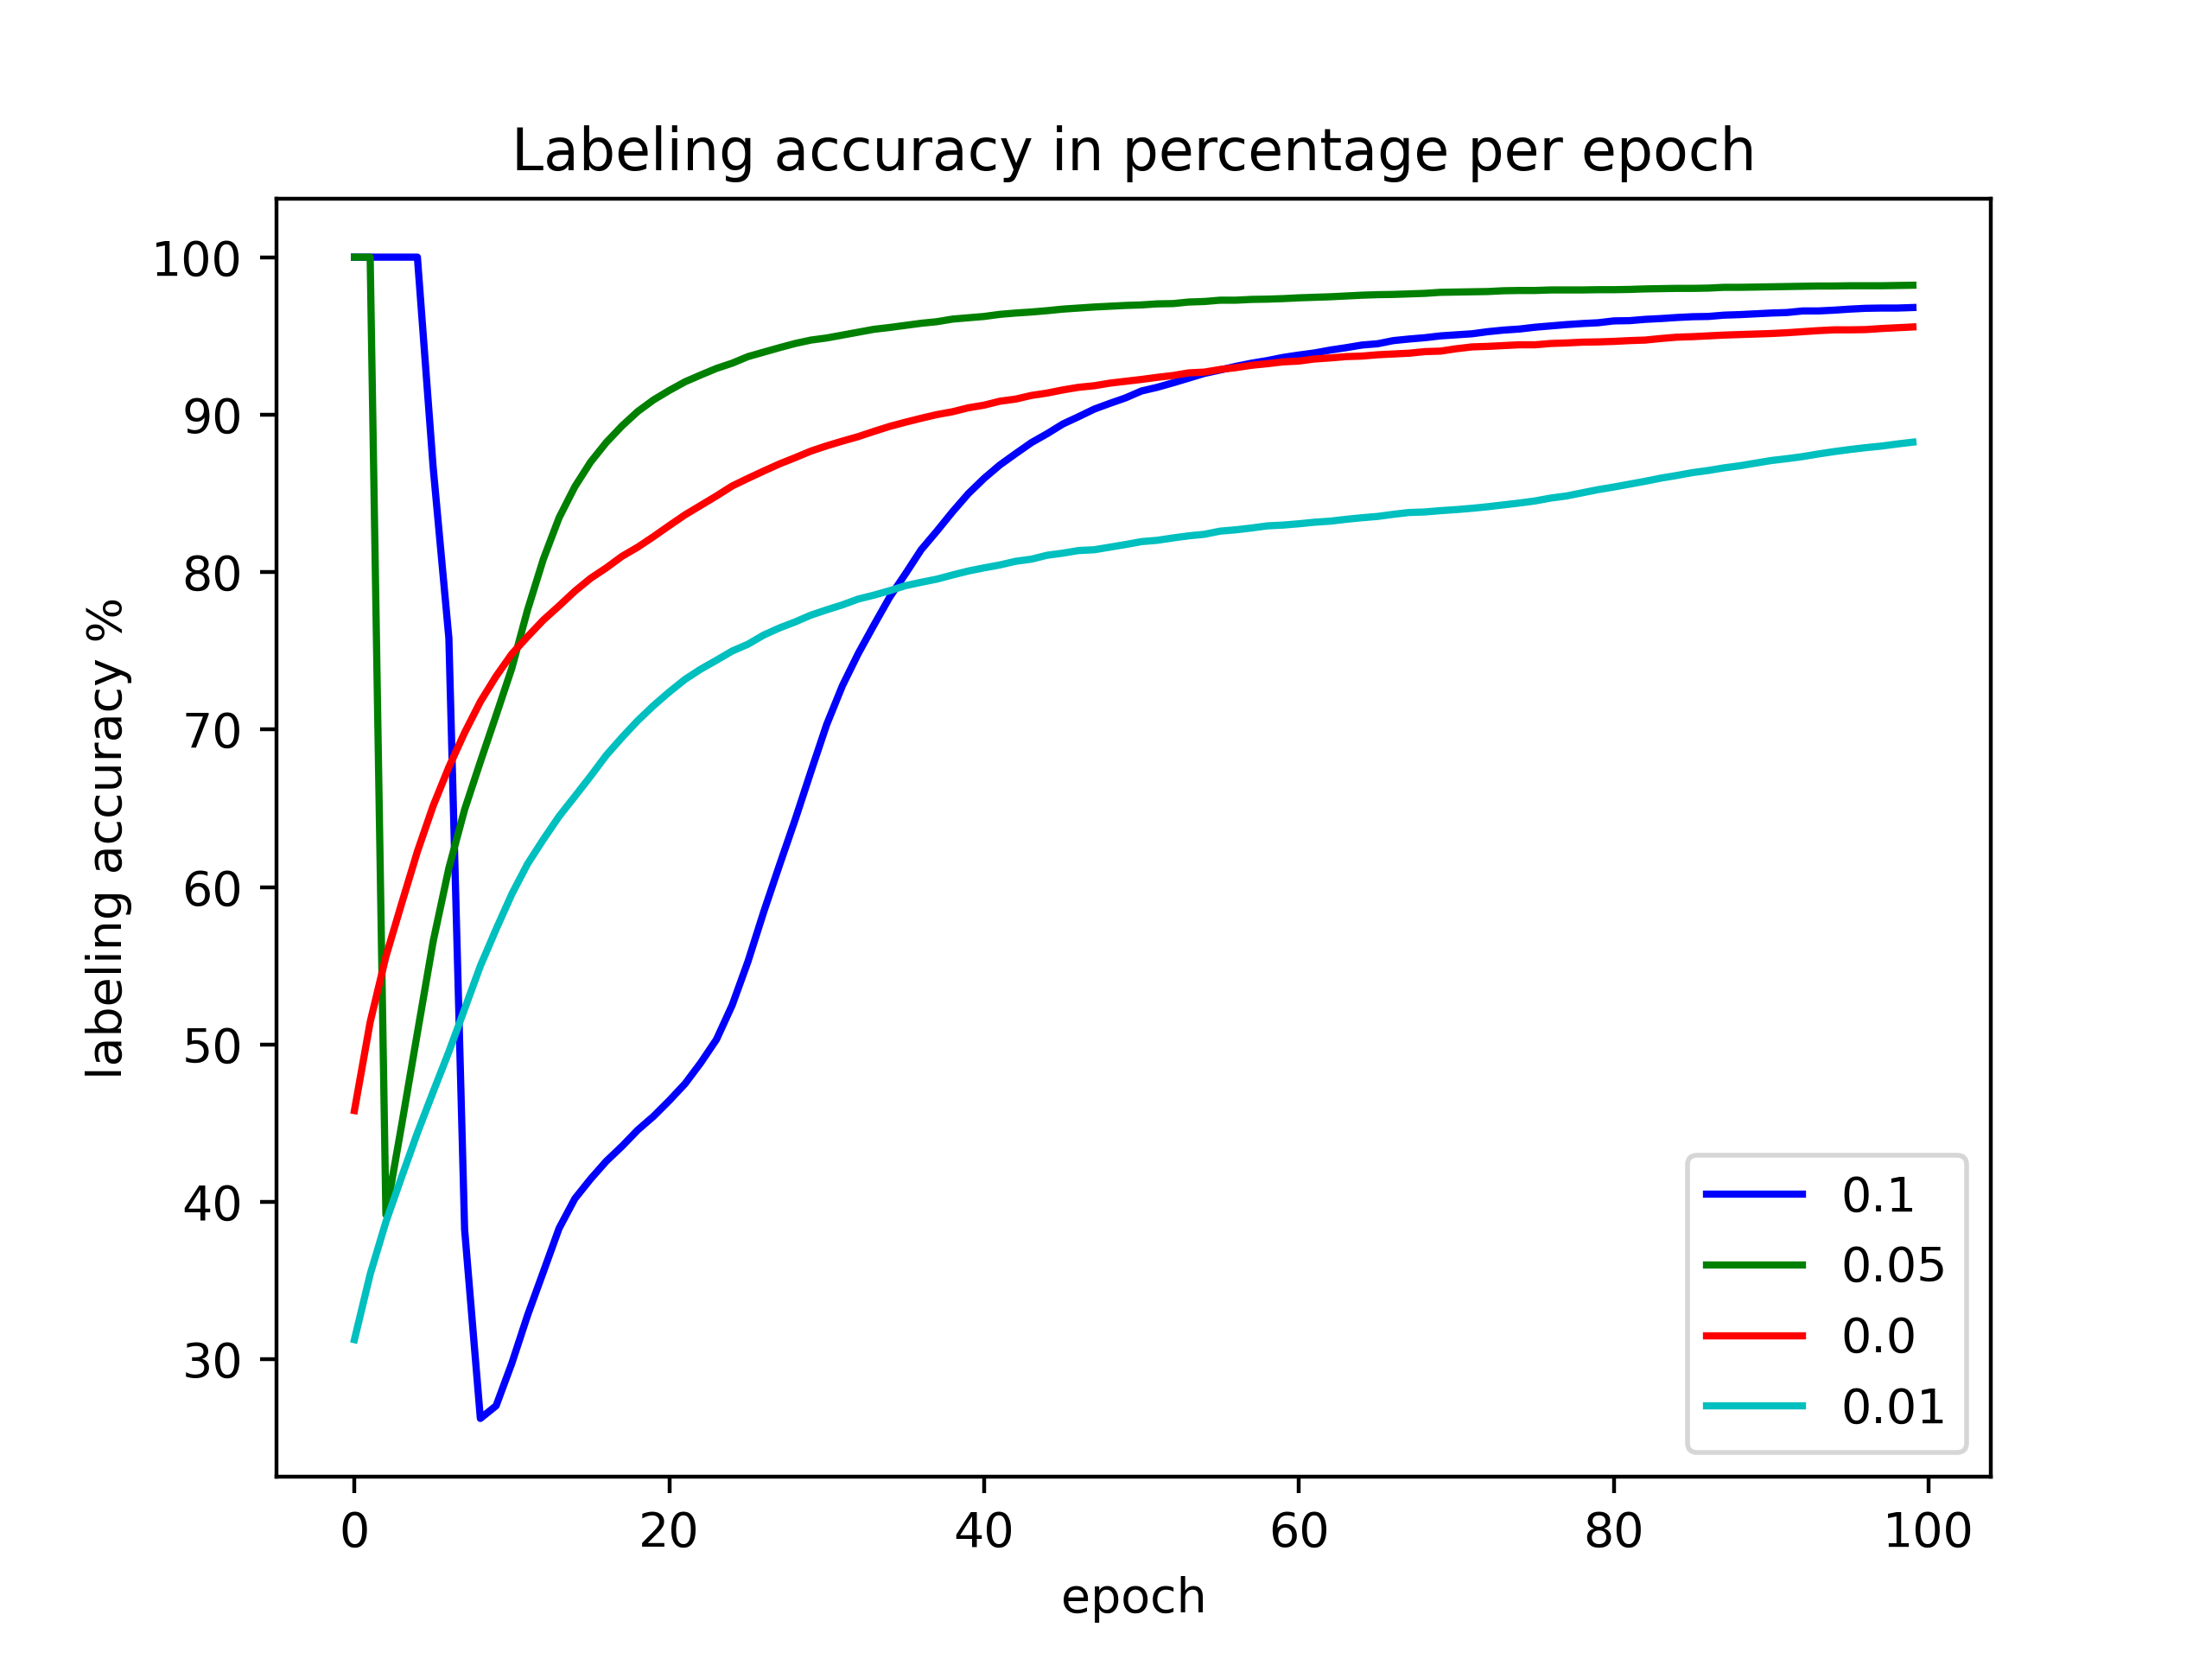
\includegraphics[scale=0.45]{Figures/num_addends_3/labeling_clno.png}} &
\subfloat{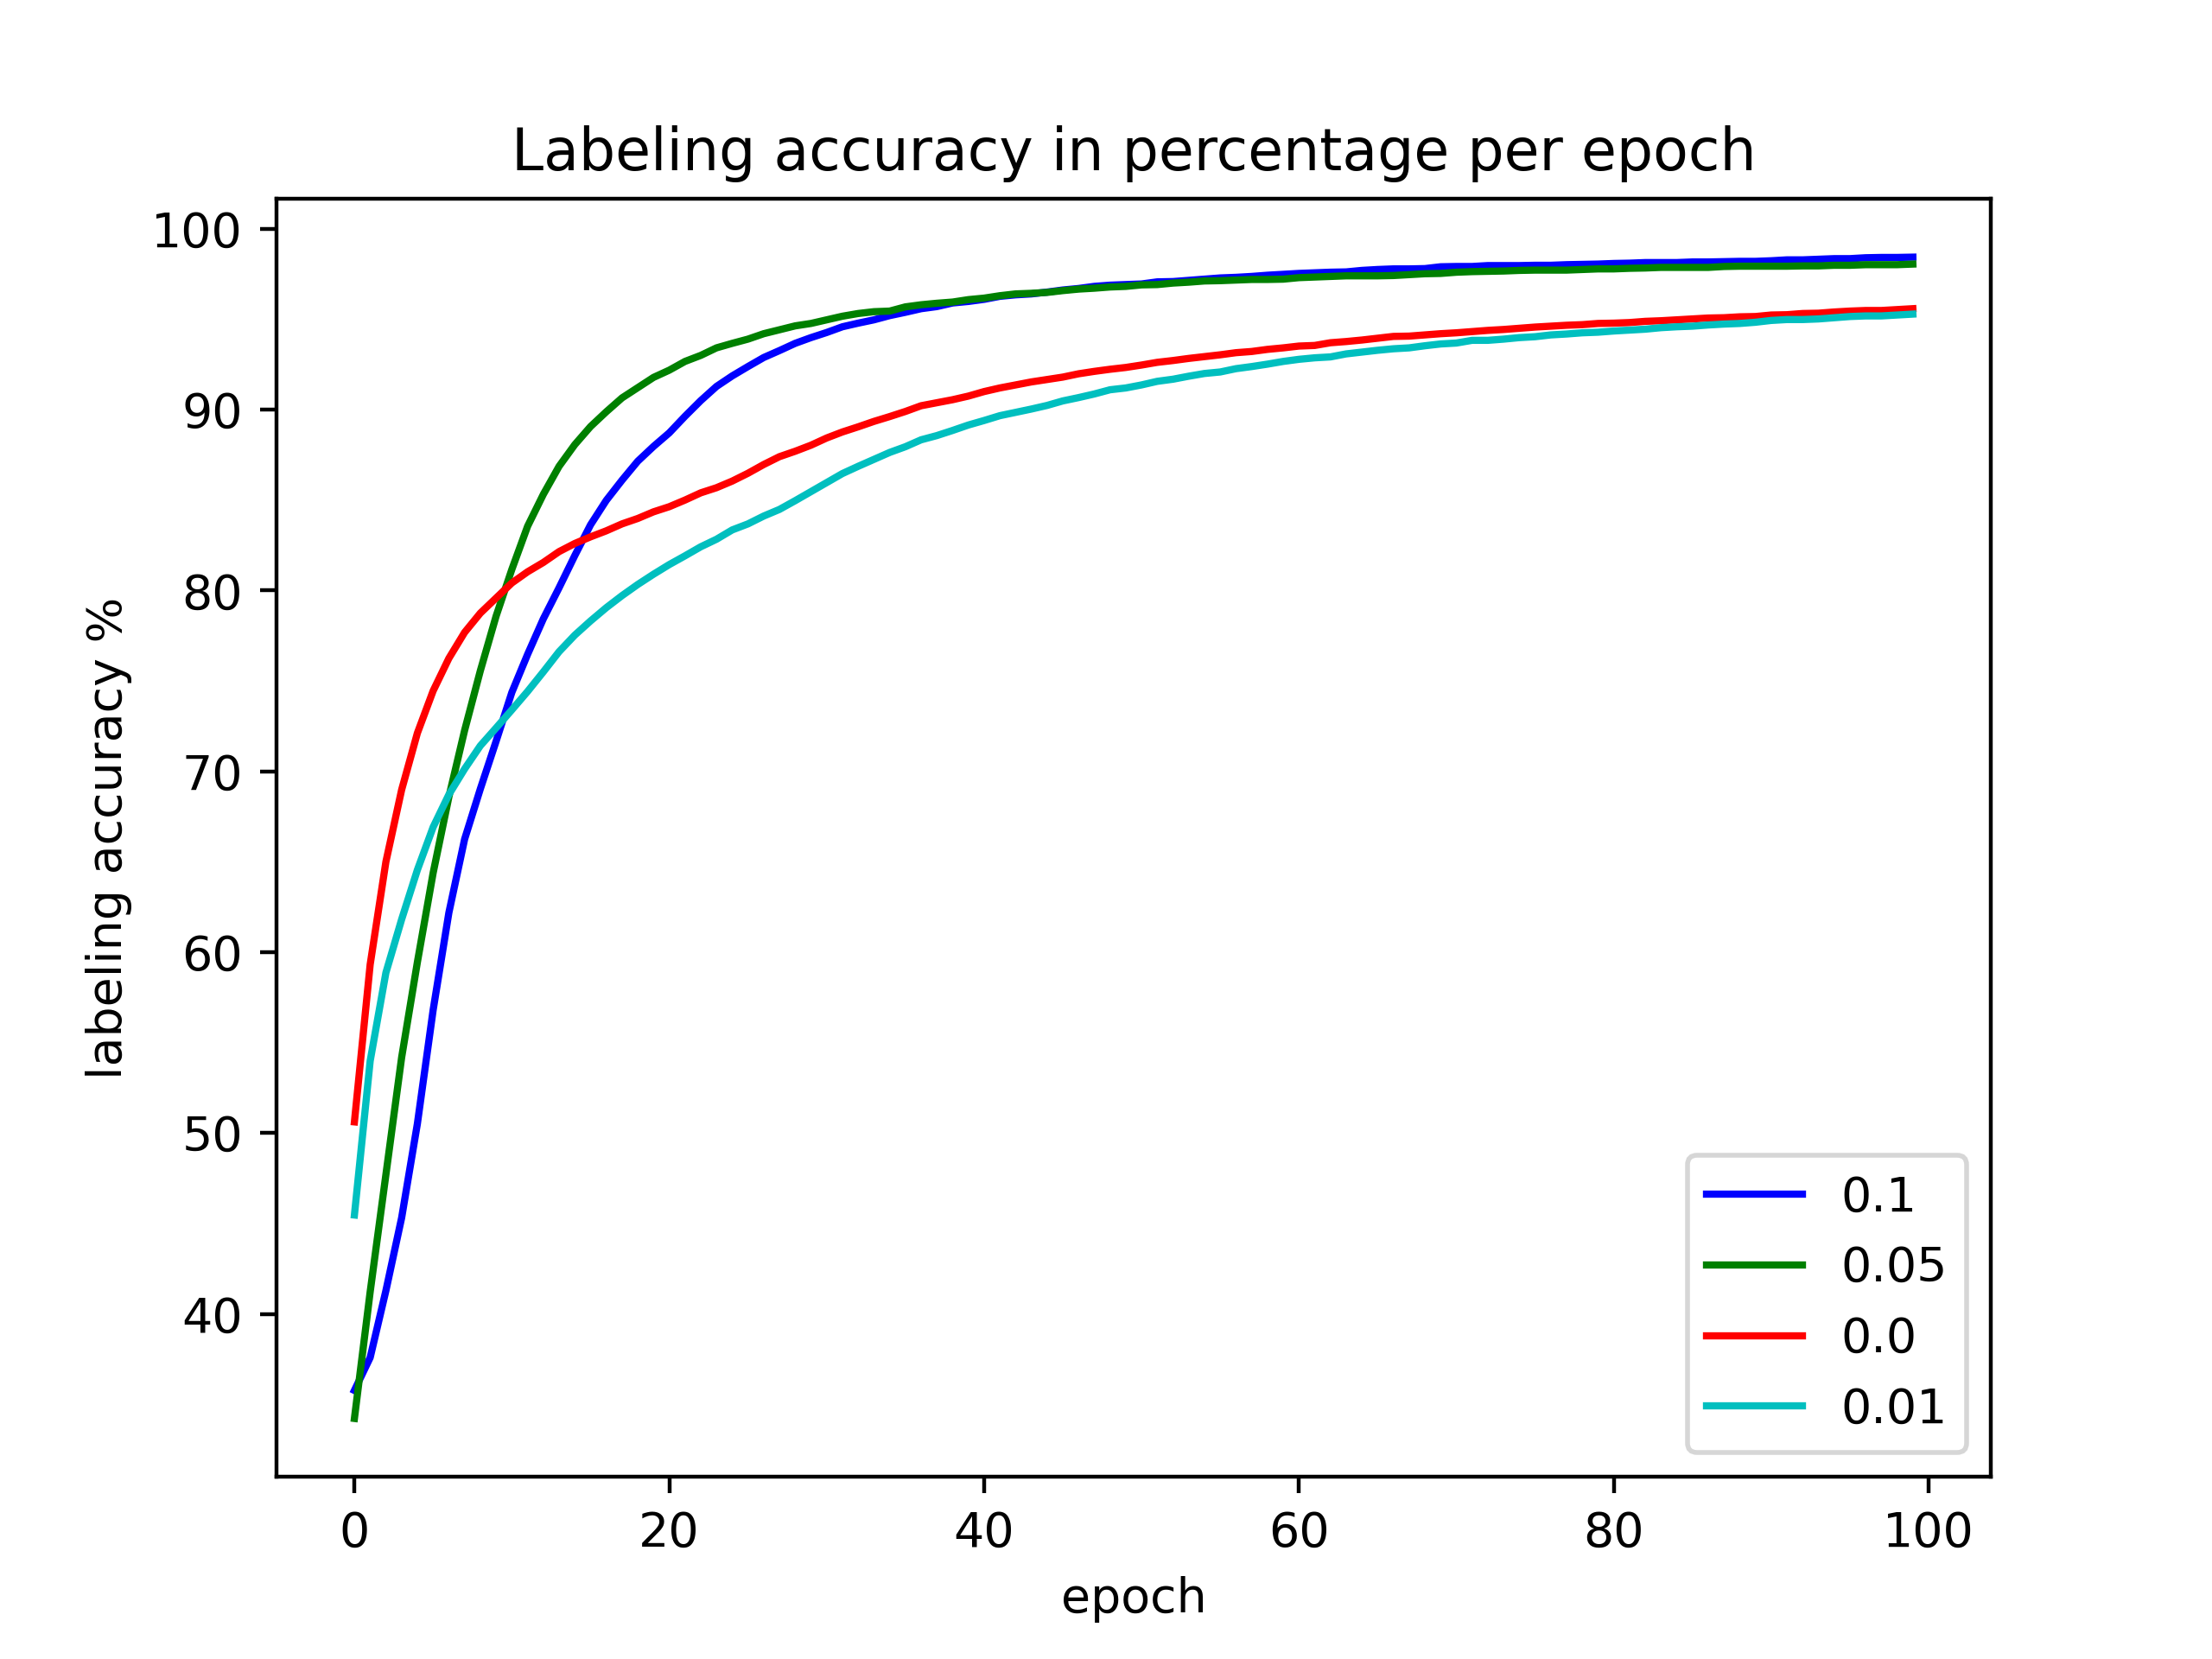
\includegraphics[scale=0.45]{Figures/num_addends_3/labeling_clyes.png}} \\

\subfloat{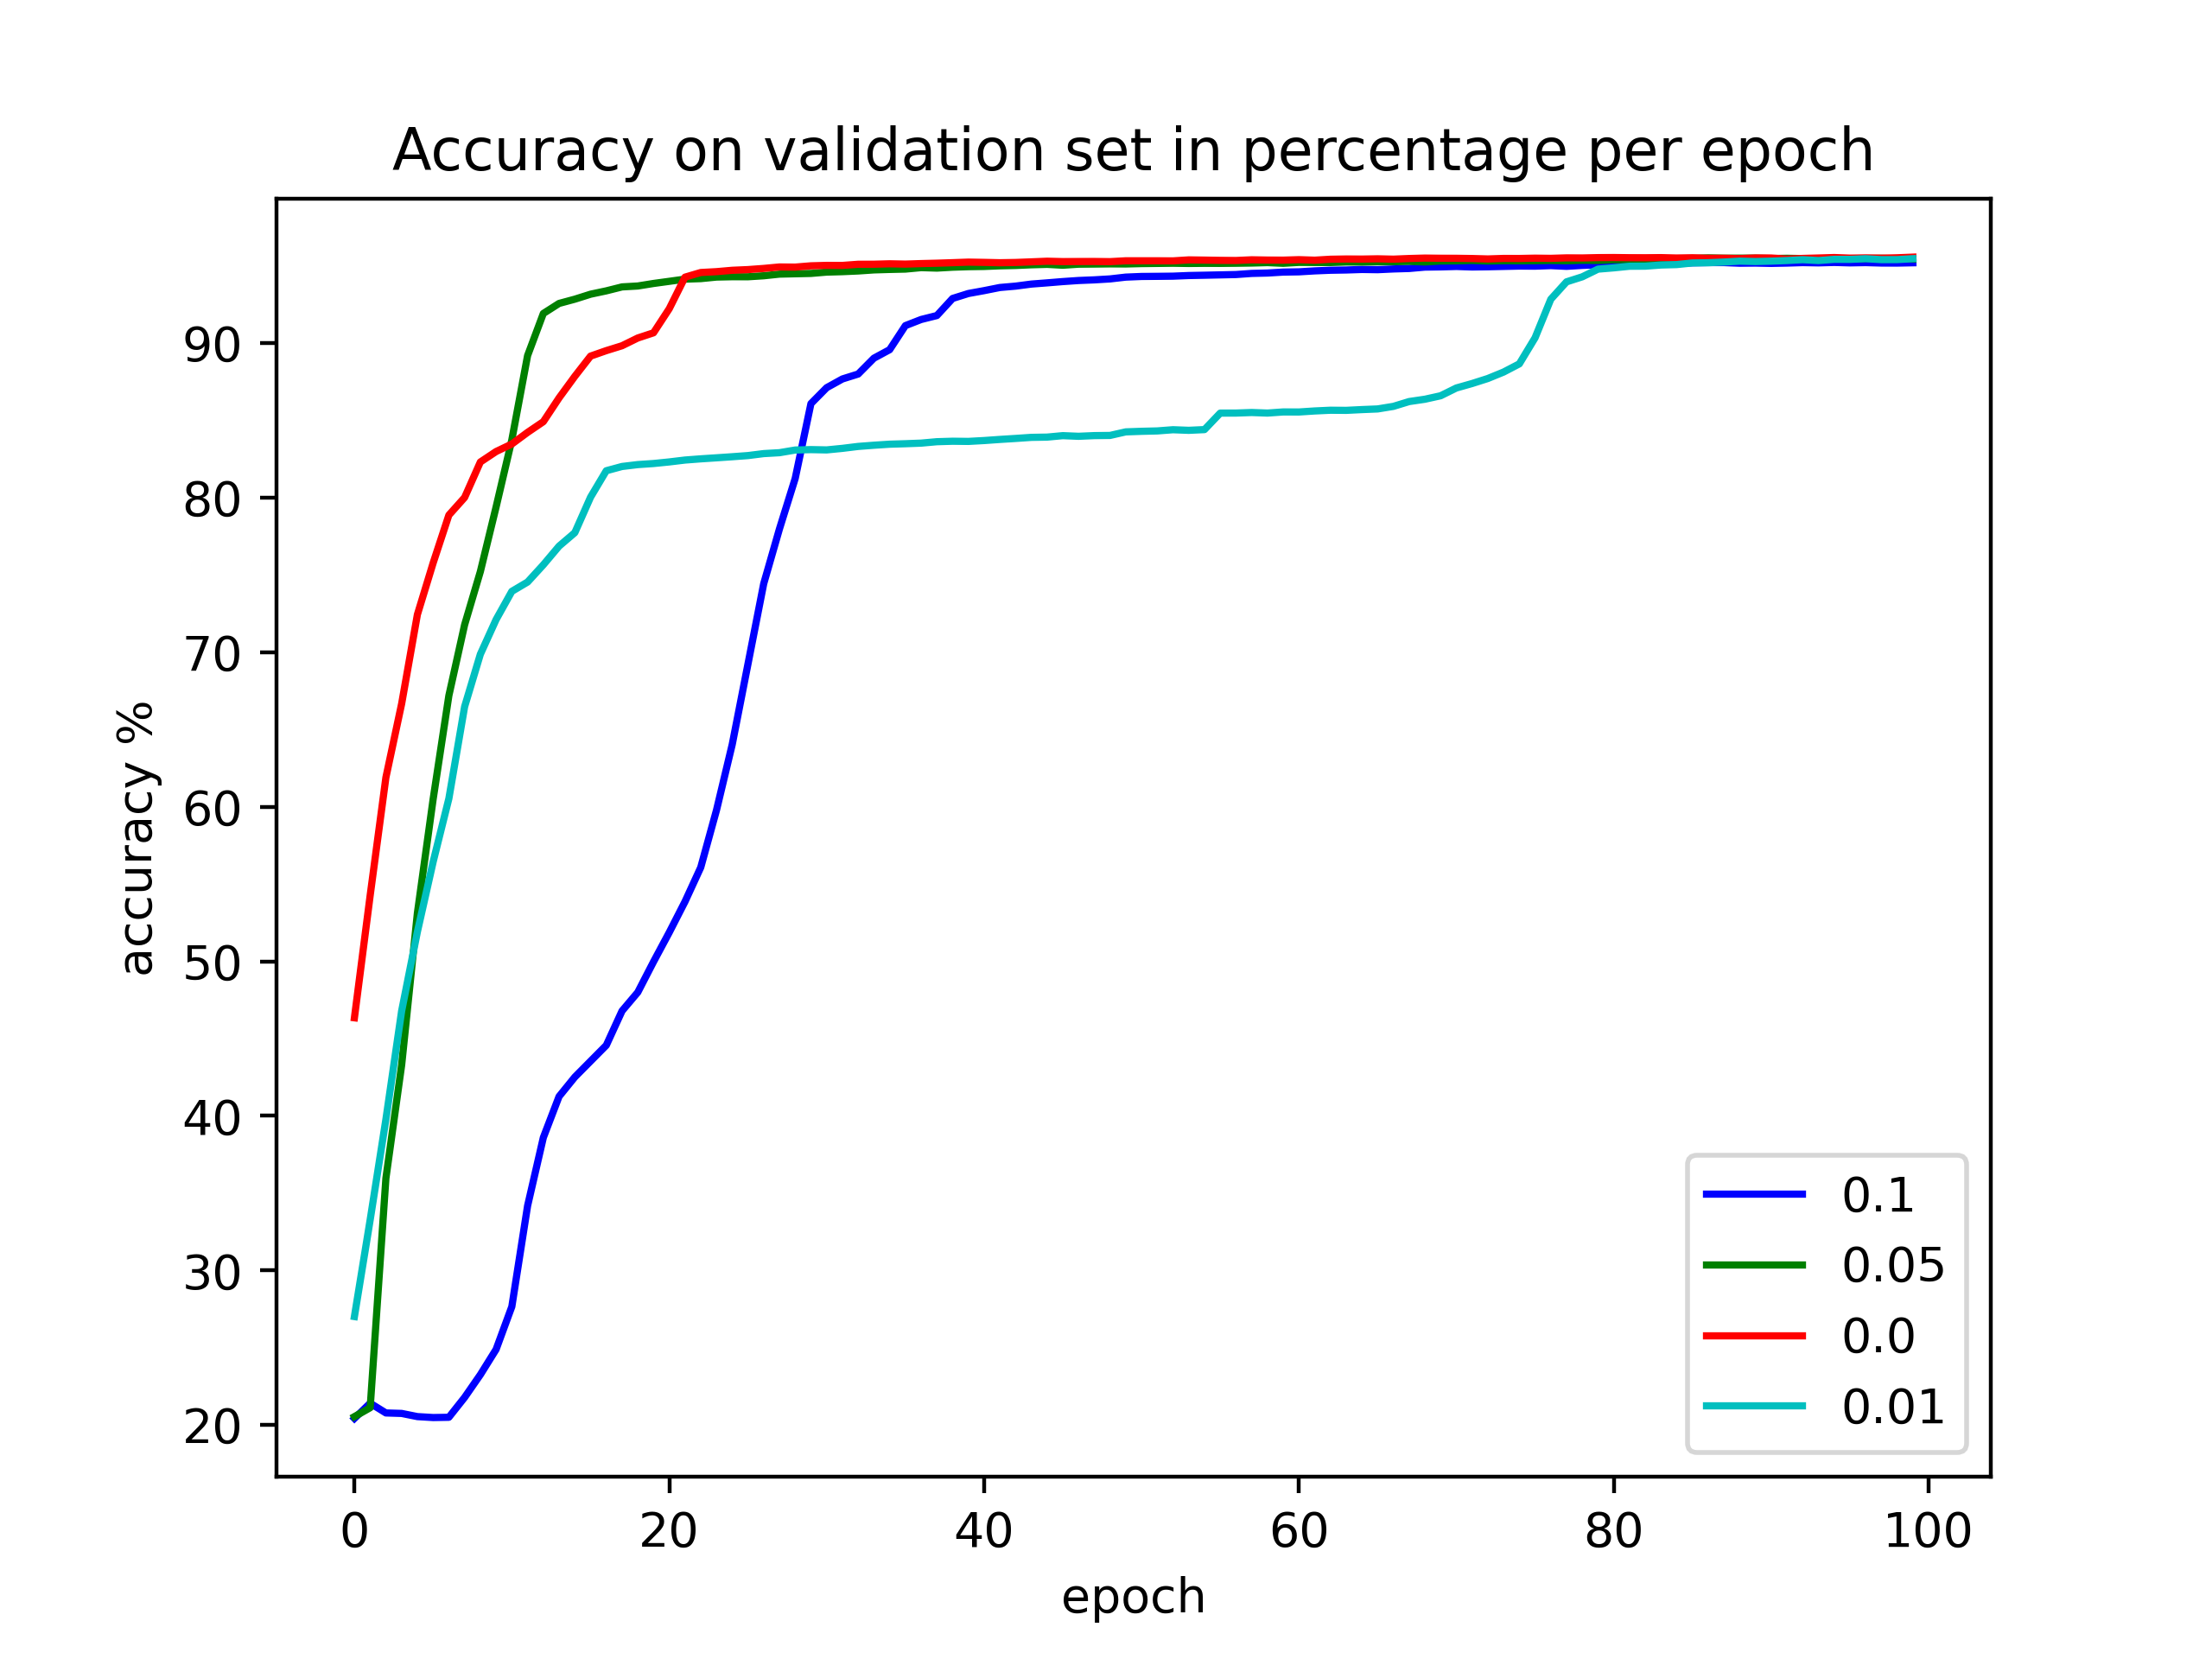
\includegraphics[scale=0.45]{Figures/num_addends_3/accuracy_clno.png}} &
\subfloat{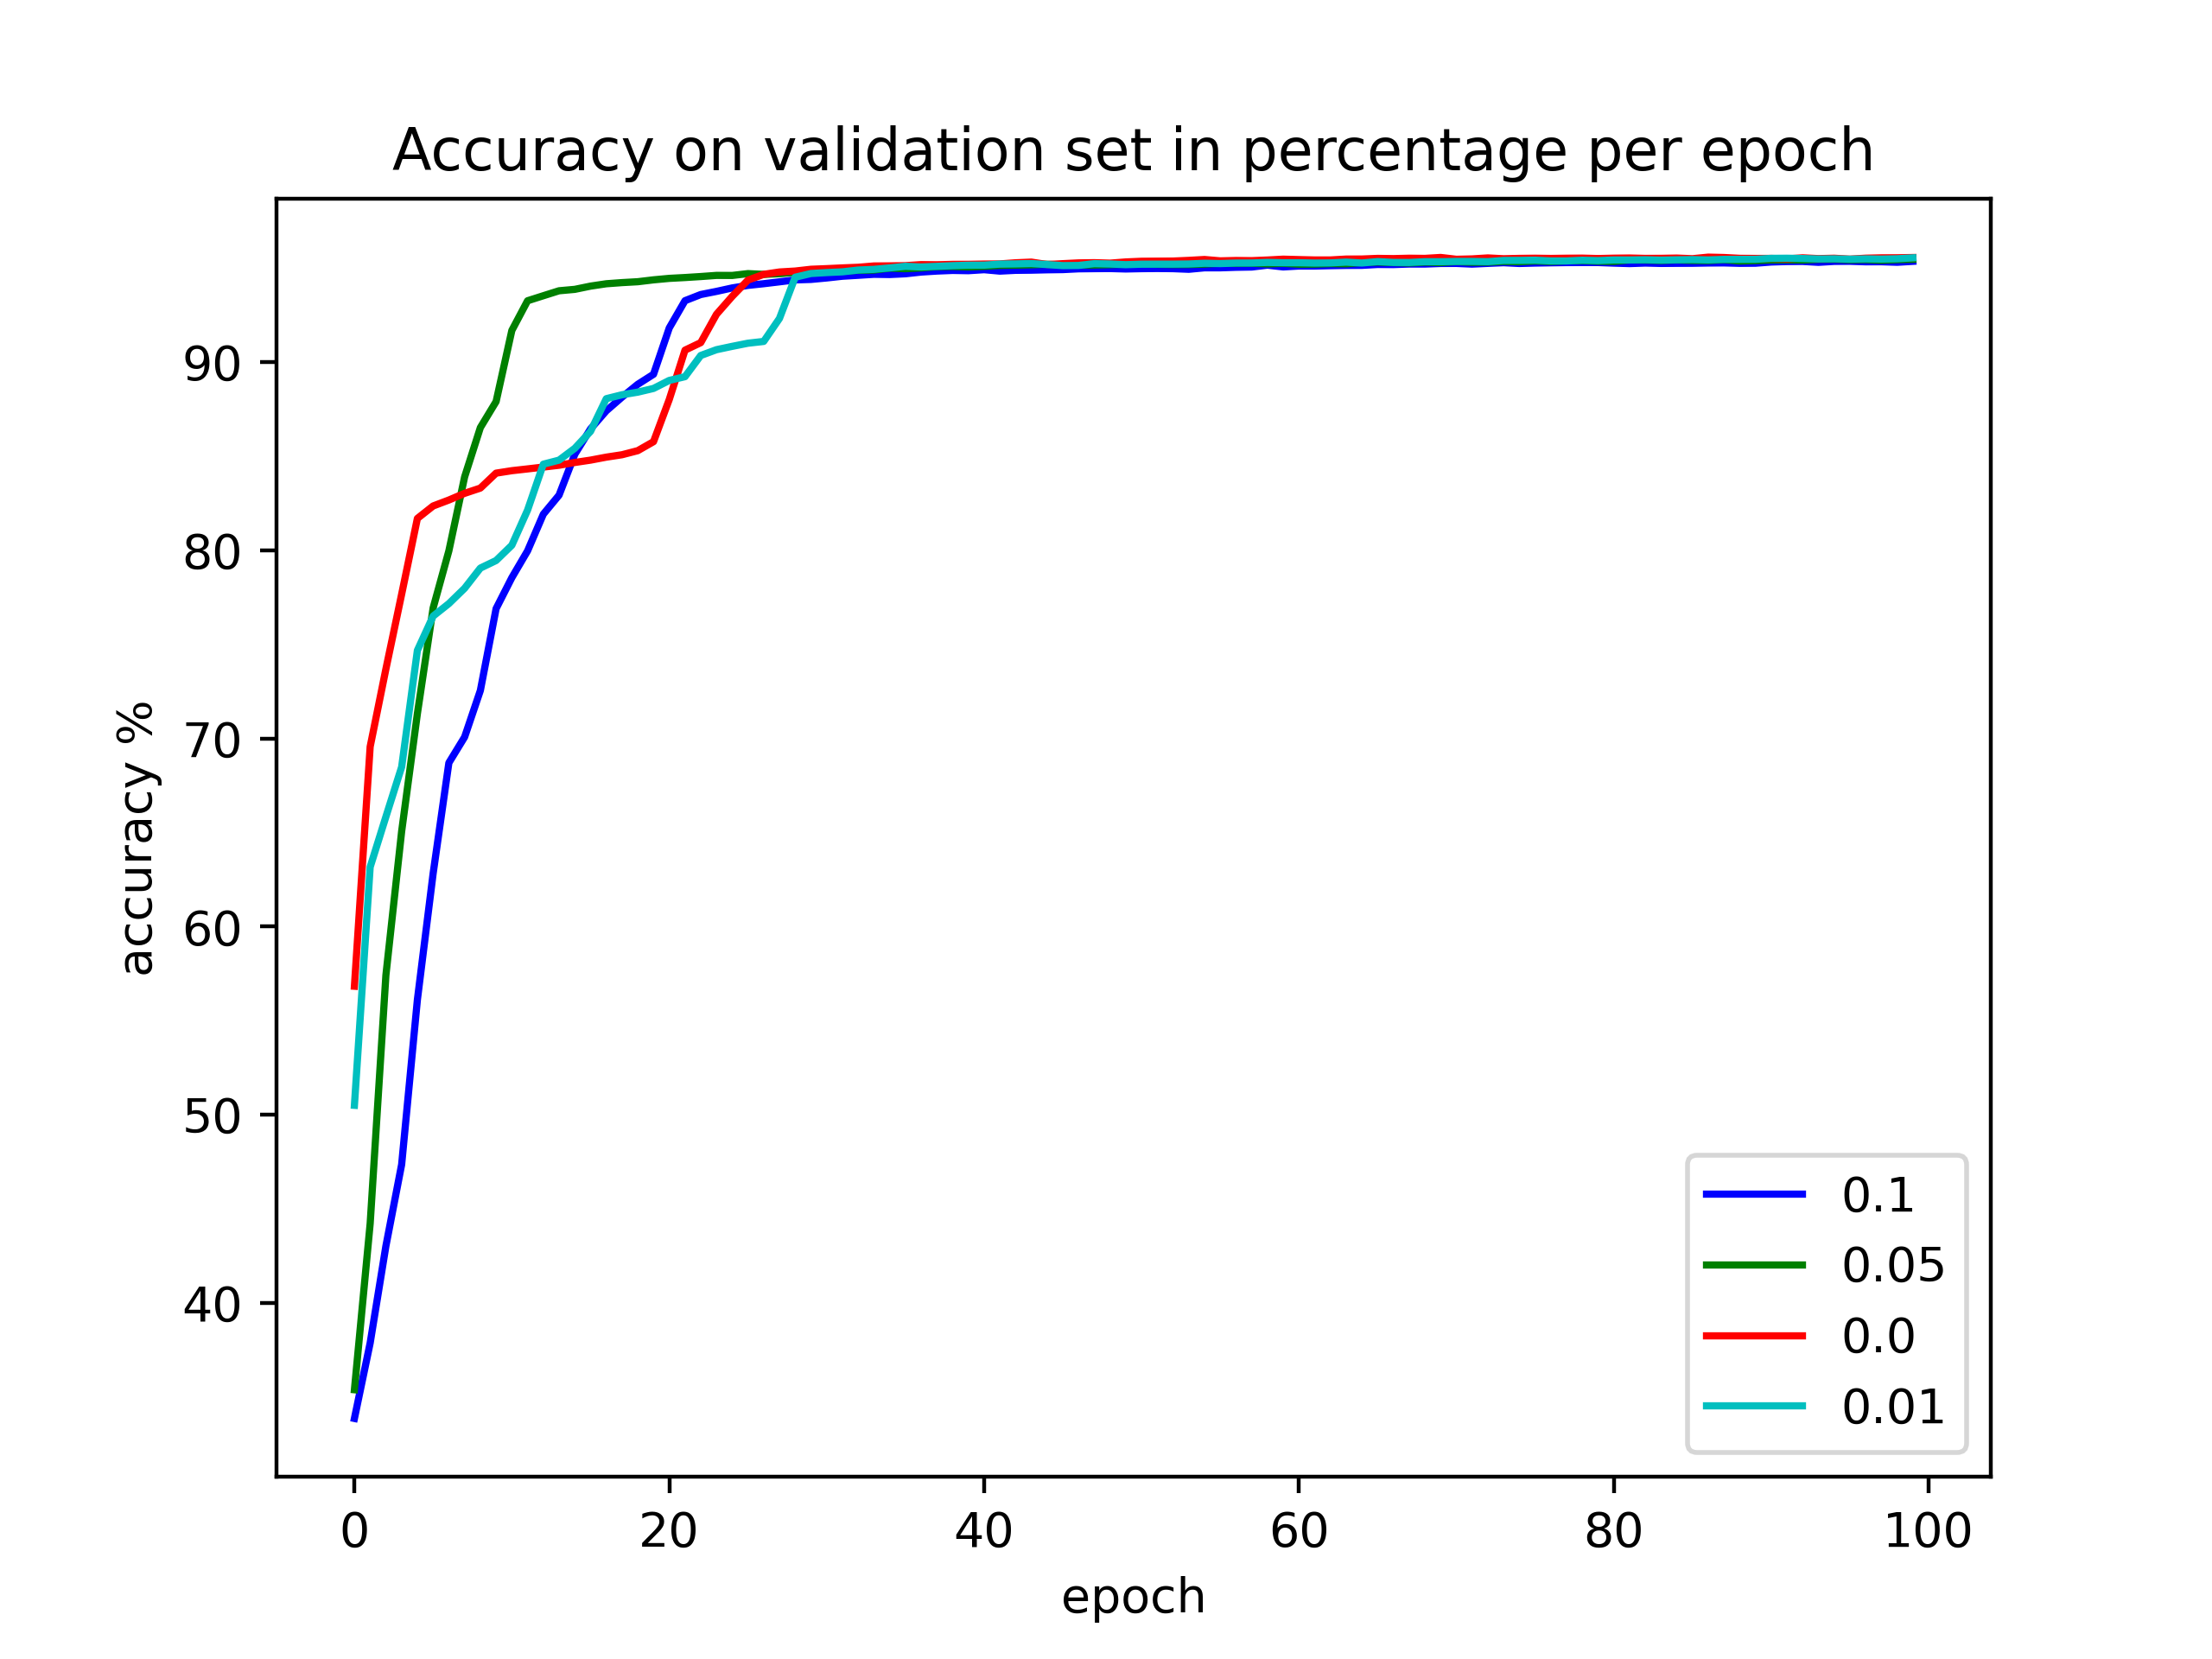
\includegraphics[scale=0.45]{Figures/num_addends_3/accuracy_clyes.png}} \\
\end{longtable}
}
\end{figure}

\subsection{Sum of quadruples}
Table \ref{tab:results-triples-clno} and \ref{tab:results-triples-clyes} show the esperiments results in the case of $m=4$ (i.e., sum of quadruples). We considered the same configurations tested for $m=3$, just slighlty increasing the threshold values. In addition, given the task extreme difficulty (see \ref{tab:info-tasks}), we also explored RAT-SPNs with split depth equal to 2 in the case of enabled pre-training.

\begin{table}[H]
  \centering
  \caption{Performance for $\mathit{f} = sum(\mathit{c}_1,\mathit{c}_2,\mathit{c}_3,\mathit{c}_4)$. Batch size = $100$, number of epochs = $100$, optimization algorithm: \textit{adam}, \textbf{pre-training = false}. All accuracy values are in percentage and approximated to the second digit after the decimal place.}
  \label{tab:results-quadruples-clno}
  \scriptsize
  \begin{tabular}{cccccccrr}
    \toprule
    depth		& distributions 	& splits 		& sums 				& dropout input 		& dropout sums 			& threshold				& valid acc 			& test acc\\
    \midrule
	1	      	& 10     			& 9      		& 10     			& 1     				& 1      				& 0  					& 25.57    				& 26.13\\ 
	1      		& 10     			& 9      		& 10    			& 1      				& 1  					& 0.05    				& 31.30    				& 32.00\\ 
	1	      	& 10     			& 9      		& 10     			& 1      				& 1  					& 0.08    				& 30.85    				& 32.41\\ 
	1   	   	& 10     			& 9      		& 10     			& 1      				& 1  					& 0.11    				& 33.02    				& 34.30\\ 
	1   	   	& 10     			& 9      		& 10 				& 0.75    				& 0.75    				& 0  					& 95.10    				& 95.16\\ 
	1      		& 10     			& 9      		& 10 				& 0.75    				& 0.75    				& 0.05    				& 93.48    				& 93.56\\ 
	1      		& 10     			& 9      		& 10 				& 0.75    				& 0.75    				& 0.08    				& 34.95    				& 35.86\\ 
	1      		& 10     			& 9      		& 10 				& 0.75    				& 0.75    				& 0.11    				& 22.92    				& 23.67\\ 
	
	1      		& 15     			& 14     		& 10     			& 1      				& 1      				& 0  					& 44.37    				& 44.59\\ 
	1      		& 15     			& 14     		& 10     			& 1      				& 1  					& 0.05    				& 25.51    				& 26.02\\ 
	1      		& 15     			& 14     		& 10     			& 1      				& 1  					& 0.08    				& 25.75    				& 26.15\\
	1      		& 15     			& 14     		& 10     			& 1      				& 1  					& 0.11    				& 29.35    				& 30.11\\ 	
	1      		& 15     			& 14     		& 10 				& 0.75    				& 0.75    				& 0						& 22.92    				& 24.03\\ 
	1      		& 15     			& 14     		& 10      			& 0.75    				& 0.75    				& 0.05    				& 25.42    				& 25.40\\ 
	1      		& 15     			& 14     		& 10 				& 0.75    				& 0.75    				& 0.08    				& 30.42    				& 31.32\\ 
	1      		& 15     			& 14     		& 10 				& 0.75    				& 0.75    				& 0.11					& 21.32    				& 21.94\\
	
	1  			& 20     			& 19			& 10				& 1						& 1      				& 0			      		& 36.21 				& 36.78\\ 
	1      		& 20     			& 19     		& 10     			& 1      				& 1      				& 0.01    				& 28.15    				& 28.99\\ 
	1      		& 20     			& 19     		& 10     			& 1      				& 1      				& 0.05    				& 35.68    				& 36.73\\
	1      		& 20     			& 19     		& 10     			& 1      				& 1      				& 0.10    				& 41.23    				& 43.58\\
	1      		& 20     			& 19     		& 10     			& 0.75      			& 0.75      			& 0	    				& 26.18    				& 26.89\\
	1      		& 20     			& 19     		& 10     			& 0.75      			& 0.75      			& 0.01    				& 93.12    				& 93.26\\
	1      		& 20     			& 19     		& 10     			& 0.75      			& 0.75      			& 0.05    				& 23.88    				& 24.00\\
	1      		& 20     			& 19     		& 10     			& 0.75      			& 0.75      			& 0.10    				& 34.11    				& 35.79\\ 
    \bottomrule
  \end{tabular}
\end{table}

\begin{table}[H]
  \centering
  \caption{Performance for $\mathit{f} = sum(\mathit{c}_1,\mathit{c}_2,\mathit{c}_3,\mathit{c}_4)$. Batch size = $100$, number of epochs = $100$, optimization algorithm: \textit{adam}, \textbf{pre-training = true}. All accuracy values are in percentage and approximated to the second digit after the decimal place.}
  \label{tab:results-quadruples-clyes}
  \scriptsize
  \begin{tabular}{cccccccrr}
    \toprule
    depth		& distributions 	& splits 		& sums 				& dropout input 		& dropout sums 			& threshold				& valid acc 			& test acc\\
    \midrule
	1 			& 10     			& 9 			& 10     			& 1 					& 1 					& 0 					& 43.92   				& 44.67\\
	1 			& 10     			& 9 			& 10     			& 1 					& 1 					& 0.05    				& 30.05    				& 31.48\\
	1 			& 10     			& 9 			& 10     			& 1 					& 1 					& 0.08    				& 28.80    				& 28.62\\
	1 			& 10     			& 9 			& 10     			& 1 					& 1 					& 0.11    				& 26.63    				& 26.67\\
	1 			& 10     			& 9 			& 10     			& 0.75    				& 0.75    				& 0 					& 96.55    				& 96.10\\
	1 			& 10     			& 9 			& 10     			& 0.75    				& 0.75    				& 0.05    				& 96.23    				& 95.79\\
	1 			& 10     			& 9 			& 10     			& 0.75    				& 0.75    				& 0.08    				& 34.78    				& 34.94\\
	1 			& 10     			& 9 			& 10     			& 0.75    				& 0.75    				& 0.11   				& 32.07    				& 31.75\\
	
	1 			& 15     			& 14     		& 10     			& 1 					& 1 					& 0 					& 94.83    				& 94.43\\
	1 			& 15     			& 14     		& 10     			& 1 					& 1 					& 0.05   				& 24.83    				& 25.73\\
	1 			& 15     			& 14     		& 10     			& 1 					& 1 					& 0.08    				& 34.62    				& 35.90\\
	1 			& 15     			& 14     		& 10     			& 1 					& 1 					& 0.11    				& 35.38    				& 35.71\\
	1 			& 15     			& 14     		& 10     			& 0.75    				& 0.75    				& 0 					& 96.05    				& 96.07\\	
	1 			& 15     			& 14     		& 10     			& 0.75    				& 0.75    				& 0.05    				& 96.35    				& 96.17\\
	1 			& 15     			& 14     		& 10     			& 0.75    				& 0.75    				& 0.08    				& 32.92    				& 33.92\\
	1 			& 15     			& 14     		& 10     			& 0.75    				& 0.75    				& 0.11   				& 27.30    				& 28.35\\

	1  			& 20     			& 19			& 10				& 1						& 1      				& 0			      		& 93.00 				& 94.12\\ 
	1      		& 20     			& 19     		& 10     			& 1      				& 1      				& 0.01    				& 31.65    				& 32.78\\ 
	1      		& 20     			& 19     		& 10     			& 1      				& 1      				& 0.05    				& 25.89    				& 26.37\\
	1      		& 20     			& 19     		& 10     			& 1      				& 1      				& 0.10    				& 44.20    				& 45.99\\
	1      		& 20     			& 19     		& 10     			& 0.75      			& 0.75      			& 0	    				& 31.54    				& 33.42\\
	1      		& 20     			& 19     		& 10     			& 0.75      			& 0.75      			& 0.01    				& 94.11    				& 95.56\\
	1      		& 20     			& 19     		& 10     			& 0.75      			& 0.75      			& 0.05    				& 28.23    				& 28.35\\
	1      		& 20     			& 19     		& 10     			& 0.75      			& 0.75      			& 0.10    				& 33.51    				& 33.93\\
	
	
	2 			& 10     			& 8 			& 10     			& 1 					& 1 					& 0 					& 19.92    				& 20.35\\
	2 			& 10     			& 8 			& 10     			& 1 					& 1 					& 0.05   				& 24.18    				& 25.09\\
	2 			& 10     			& 8 			& 10     			& 1 					& 1 					& 0.08    				& 32.20    				& 33.14\\
	2 			& 10     			& 8 			& 10     			& 1 					& 1 					& 0.11    				& 37.87    				& 37.39\\	
	2 			& 10     			& 8 			& 10     			& 0.75    				& 0.75    				& 0 					& 97.60    				& 97.15\\
	2 			& 10     			& 8 			& 10     			& 0.75    				& 0.75    				& 0.05    				& 33.80    				& 33.48\\
	2 			& 10     			& 8 			& 10     			& 0.75    				& 0.75    				& 0.08    				& 36.53    				& 36.09\\
	2 			& 10     			& 8 			& 10     			& 0.75    				& 0.75    				& 0.11    				& 37.98    				& 38.01\\

	2 			& 15     			& 12     		& 15     			& 1 					& 1 					& 0 					& 20.73    				& 21.00\\
	2 			& 15     			& 12     		& 15     			& 1 					& 1 					& 0.05    				& 25.07    				& 25.58\\
	2 			& 15     			& 12     		& 15     			& 1 					& 1 					& 0.08    				& 33.50    				& 34.02\\
	2 			& 15     			& 12     		& 15     			& 1 					& 1 					& 0.11    				& 39.42    				& 40.47\\
	2 			& 15     			& 12     		& 15     			& 0.75    				& 0.75    				& 0 					& 26.00    	 			& 26.81\\
	2 			& 15     			& 12     		& 15     			& 0.75    				& 0.75    				& 0.08    				& 37.48    				& 38.26\\
	2 			& 15     			& 12     		& 15     			& 0.75    				& 0.75    				& 0.05    				& 27.82    				& 28.84\\
	2 			& 15     			& 12     		& 15     			& 0.75    				& 0.75    				& 0.11    				& 41.52    				& 42.50\\
    \bottomrule
  \end{tabular}
\end{table}
Unfortunately, the behaviour shown by the above tables is similar to the one highlighted in Table \ref{tab:simple-model}: performance varies greatly from one configuration to another, indicating that the lerning is no longer deterministic, but prone to chance. Nevertheless, with respect to Table \ref{tab:simple-model}, we note a significant difference: there are no "intermediate" accuracy values, basically the model converges or doesn't learn at all. This could mean that, if the model "finds the correct direction", it is always able to converge and achieve good performance.

Given the non-deterministic nature of learning, in this case it is not interesting to evaluate the model behaviour as in Figures \ref{fig:thresholds-triples}. Nevertheless, we want to understand if the pre-training can still bring some advantages. For this purpose, Table \ref{tab:comparison-pre-training} compares corresponding configurations (with depth equal to 1) of the pre-trained model and the not pre-trained one, taking into account \textit{(i)} the number of considered examples and \textit{(ii)} the ratios of examples labeling accuracy of digit from 0 to 2. The analysis is limited to the first epoch, because it is the most influenced by the pre-training, and to such digits, because we observed that the pre-training perform only on \textit{zero} examples (for this specific task). Results highlighted by such analysis are evident: the examples labeling accuracy is always higher when the pre-training is enabled, except for two not relevant cases in which it is slighlty lower, but in the face of a greater number of considered examples.

We can conclude that the pre-training still correctly works, but it is no longer sufficient, in conjunction with the abduction threshold, to solve such a difficult task. 

\begin{table}[H]
  \centering
  \caption{Comparison between corresponding configurations (with split depth = 1) of the pre-trained model and the not pre-trained one, with reference to Tables \ref{tab:results-quadruples-clno} and \ref{tab:results-quadruples-clyes}. \#(examples) refers to the number of considered examples during the current training epoch, while $R_i$ refers to the ratio of examples labeling accuracy of the \textit{i-th} digit. All the reported values refer to the \textbf{first} training epoch. Greater $R_i$ values between corresponding configurations are highlighted in bold.}
  \label{tab:comparison-pre-training}
  \small
  \begin{tabular}{cccc|cccc}
	\multicolumn{4}{c|}{\textbf{Pre-training = true}} & \multicolumn{4}{c}{\textbf{Pre-training = false}}\\
	\hline
	\multicolumn{1}{c}{\#(examples)} & $R_0$ & $R_1$ & $R_2$ & 
	\multicolumn{1}{c}{\#(examples)} & $R_0$ & $R_1$ & \multicolumn{1}{c}{$R_2$} \\
	\hline
	54000	& \textbf{0.90}	& \textbf{0.89}	& \textbf{0.06}	& 54000	& 0.64	& 0.02	& 0.05 \\
	32		& 0.95	& 0.33	& -		& 12	& \textbf{1}	& -		& - \\
	12		& 1		& -		& -		& 12	& 1		& -		& - \\
	12		& 1		& -		& -		& 12	& 1		& -		& - \\
	54000	& \textbf{0.93}	& \textbf{0.86}	& \textbf{0.14}	& 54000	& 0.83	& 0.05	& 0.08 \\
	36		& 1		& \textbf{1}		& -	& 12	& 1		& -		& - \\
	12		& 1		& -		& -		& 12	& 1		& -		& - \\
	12		& 1		& -		& -		& 12	& 1		& -		& - \\
	
	54000	& \textbf{0.90}	& \textbf{0.81}	& \textbf{0.13}	& 54000 & 0.89	& 0.14	& 0.08 \\
	52		& 1		& 0.33	& 0.67	& 12	& 1		& -		& - \\
	12		& 1		& -		& -		& 12	& 1		& -		& - \\
	12		& 1		& -		& -		& 12	& 1		& -		& - \\
	54000	& \textbf{0.89}	& \textbf{0.94}	& \textbf{0.31}	& 54000 & 0.88	& 0.85	& 0.06 \\
	12		& 1		& -		& -		& 12	& 1		& -		& - \\
	12		& 1		& -		& -		& 12	& 1		& -		& - \\
	12		& 1		& -		& -		& 12	& 1		& -		& - \\
	
	54000	& \textbf{0.91}	& \textbf{0.88}	& \textbf{0.12}	& 54000	& 0.60	& 0.06	& 0.02 \\
	40		& 0.97	& 0.41	& -		& 12	& \textbf{1}	& -		& - \\
	12		& 1		& -		& -		& 12	& 1		& -		& - \\
	12		& 1		& -		& -		& 12	& 1		& -		& - \\
	54000	& \textbf{0.92}	& \textbf{0.85}	& \textbf{0.12}	& 54000	& 0.79	& 0.25	& 0.04 \\
	12		& 1		& -		& -		& 12	& 1		& -		& - \\
	12		& 1		& -		& -		& 12	& 1		& -		& - \\
	12		& 1		& -		& -		& 12	& 1		& -		& - \\
   \end{tabular}
\end{table}